\documentclass[12pt,a4paper,fleqn,leqno]{article}
\usepackage{mathtext}
\usepackage{cmap}
\usepackage[utf8x]{inputenc}
\usepackage[russian]{babel}
\usepackage[T2A]{fontenc}
\usepackage{amsmath,amssymb,amsthm,amscd,amsfonts}
\usepackage{euscript}
\usepackage{relsize}
\usepackage{mathdots}
\usepackage{graphicx}
\usepackage{epstopdf}
\usepackage{caption2}
\usepackage{indentfirst}
\usepackage{fancyhdr}
\usepackage{sectsty}
\usepackage{titlesec}
\usepackage{sicpro_rus}
\usepackage{mathtext}%русские буквы в формулах

\usepackage[colorlinks, urlcolor=blue, pdfborder={0 0 0 [0 0]}]{hyperref}

\hyphenation{Struc-tu-red}
\hyphenation{Ran-do-mized}
\hyphenation{Ma-xi-mi-za-tion}
\DeclareMathOperator*{\argmax}{arg\,max}
\DeclareMathOperator*{\argmin}{arg\,min}
\DeclareMathOperator{\tr}{tr}

\def\rank{\mathop{\mathrm{rank}}}
\newtheorem{corollary}{Следствие}
\newtheorem{proposition}{Предложение}
\newtheorem{algorithm}{Алгоритм}
\newtheorem{lemma}{Лемма}

%new calligraphic font for subspaces
\usepackage{euscript}
\newcommand{\spA}{\EuScript{A}}
\newcommand{\spB}{\EuScript{B}}
\newcommand{\spC}{\EuScript{C}}
\newcommand{\spD}{\EuScript{D}}
\newcommand{\spE}{\EuScript{E}}
\newcommand{\spF}{\EuScript{F}}
\newcommand{\spG}{\EuScript{G}}
\newcommand{\spH}{\EuScript{H}}
\newcommand{\spI}{\EuScript{I}}
\newcommand{\spJ}{\EuScript{J}}
\newcommand{\spK}{\EuScript{K}}
\newcommand{\spL}{\EuScript{L}}
\newcommand{\spM}{\EuScript{M}}
\newcommand{\spN}{\EuScript{N}}
\newcommand{\spO}{\EuScript{O}}
\newcommand{\spP}{\EuScript{P}}
\newcommand{\spQ}{\EuScript{Q}}
\newcommand{\spR}{\EuScript{R}}
\newcommand{\spS}{\EuScript{S}}
\newcommand{\spT}{\EuScript{T}}
\newcommand{\spU}{\EuScript{U}}
\newcommand{\spV}{\EuScript{V}}
\newcommand{\spW}{\EuScript{W}}
\newcommand{\spX}{\EuScript{X}}
\newcommand{\spY}{\EuScript{Y}}
\newcommand{\spZ}{\EuScript{Z}}

%font for text indices like transposition X^\mathrm{T}
\newcommand{\rmA}{\mathrm{A}}
\newcommand{\rmB}{\mathrm{B}}
\newcommand{\rmC}{\mathrm{C}}
\newcommand{\rmD}{\mathrm{D}}
\newcommand{\rmE}{\mathrm{E}}
\newcommand{\rmF}{\mathrm{F}}
\newcommand{\rmG}{\mathrm{G}}
\newcommand{\rmH}{\mathrm{H}}
\newcommand{\rmI}{\mathrm{I}}
\newcommand{\rmJ}{\mathrm{J}}
\newcommand{\rmK}{\mathrm{K}}
\newcommand{\rmL}{\mathrm{L}}
\newcommand{\rmM}{\mathrm{M}}
\newcommand{\rmN}{\mathrm{N}}
\newcommand{\rmO}{\mathrm{O}}
\newcommand{\rmP}{\mathrm{P}}
\newcommand{\rmQ}{\mathrm{Q}}
\newcommand{\rmR}{\mathrm{R}}
\newcommand{\rmS}{\mathrm{S}}
\newcommand{\rmT}{\mathrm{T}}
\newcommand{\rmU}{\mathrm{U}}
\newcommand{\rmV}{\mathrm{V}}
\newcommand{\rmW}{\mathrm{W}}
\newcommand{\rmX}{\mathrm{X}}
\newcommand{\rmY}{\mathrm{Y}}
\newcommand{\rmZ}{\mathrm{Z}}

%tt font for time series
\newcommand{\tsA}{\mathbb{A}}
\newcommand{\tsB}{\mathbb{B}}
\newcommand{\tsC}{\mathbb{C}}
\newcommand{\tsD}{\mathbb{D}}
\newcommand{\tsE}{\mathbb{E}}
\newcommand{\tsF}{\mathbb{F}}
\newcommand{\tsG}{\mathbb{G}}
\newcommand{\tsH}{\mathbb{H}}
\newcommand{\tsI}{\mathbb{I}}
\newcommand{\tsJ}{\mathbb{J}}
\newcommand{\tsK}{\mathbb{K}}
\newcommand{\tsL}{\mathbb{L}}
\newcommand{\tsM}{\mathbb{M}}
\newcommand{\tsN}{\mathbb{N}}
\newcommand{\tsO}{\mathbb{O}}
\newcommand{\tsP}{\mathbb{P}}
\newcommand{\tsQ}{\mathbb{Q}}
\newcommand{\tsR}{\mathbb{R}}
\newcommand{\tsS}{\mathbb{S}}
\newcommand{\tsT}{\mathbb{T}}
\newcommand{\tsU}{\mathbb{U}}
\newcommand{\tsV}{\mathbb{V}}
\newcommand{\tsW}{\mathbb{W}}
\newcommand{\tsX}{\mathbb{X}}
\newcommand{\tsY}{\mathbb{Y}}
\newcommand{\tsZ}{\mathbb{Z}}

%bf font for matrices
\newcommand{\bfA}{\mathbf{A}}
\newcommand{\bfB}{\mathbf{B}}
\newcommand{\bfC}{\mathbf{C}}
\newcommand{\bfD}{\mathbf{D}}
\newcommand{\bfE}{\mathbf{E}}
\newcommand{\bfF}{\mathbf{F}}
\newcommand{\bfG}{\mathbf{G}}
\newcommand{\bfH}{\mathbf{H}}
\newcommand{\bfI}{\mathbf{I}}
\newcommand{\bfJ}{\mathbf{J}}
\newcommand{\bfK}{\mathbf{K}}
\newcommand{\bfL}{\mathbf{L}}
\newcommand{\bfM}{\mathbf{M}}
\newcommand{\bfN}{\mathbf{N}}
\newcommand{\bfO}{\mathbf{O}}
\newcommand{\bfP}{\mathbf{P}}
\newcommand{\bfQ}{\mathbf{Q}}
\newcommand{\bfR}{\mathbf{R}}
\newcommand{\bfS}{\mathbf{S}}
\newcommand{\bfT}{\mathbf{T}}
\newcommand{\bfU}{\mathbf{U}}
\newcommand{\bfV}{\mathbf{V}}
\newcommand{\bfW}{\mathbf{W}}
\newcommand{\bfX}{\mathbf{X}}
\newcommand{\bfY}{\mathbf{Y}}
\newcommand{\bfZ}{\mathbf{Z}}

%bb font for standard spaces and expectation
\newcommand{\bbA}{\mathbb{A}}
\newcommand{\bbB}{\mathbb{B}}
\newcommand{\bbC}{\mathbb{C}}
\newcommand{\bbD}{\mathbb{D}}
\newcommand{\bbE}{\mathbb{E}}
\newcommand{\bbF}{\mathbb{F}}
\newcommand{\bbG}{\mathbb{G}}
\newcommand{\bbH}{\mathbb{H}}
\newcommand{\bbI}{\mathbb{I}}
\newcommand{\bbJ}{\mathbb{J}}
\newcommand{\bbK}{\mathbb{K}}
\newcommand{\bbL}{\mathbb{L}}
\newcommand{\bbM}{\mathbb{M}}
\newcommand{\bbN}{\mathbb{N}}
\newcommand{\bbO}{\mathbb{O}}
\newcommand{\bbP}{\mathbb{P}}
\newcommand{\bbQ}{\mathbb{Q}}
\newcommand{\bbR}{\mathbb{R}}
\newcommand{\bbS}{\mathbb{S}}
\newcommand{\bbT}{\mathbb{T}}
\newcommand{\bbU}{\mathbb{U}}
\newcommand{\bbV}{\mathbb{V}}
\newcommand{\bbW}{\mathbb{W}}
\newcommand{\bbX}{\mathbb{X}}
\newcommand{\bbY}{\mathbb{Y}}
\newcommand{\bbZ}{\mathbb{Z}}

%got font for any case
\newcommand{\gA}{\mathfrak{A}}
\newcommand{\gB}{\mathfrak{B}}
\newcommand{\gC}{\mathfrak{C}}
\newcommand{\gD}{\mathfrak{D}}
\newcommand{\gE}{\mathfrak{E}}
\newcommand{\gF}{\mathfrak{F}}
\newcommand{\gG}{\mathfrak{G}}
\newcommand{\gH}{\mathfrak{H}}
\newcommand{\gI}{\mathfrak{I}}
\newcommand{\gJ}{\mathfrak{J}}
\newcommand{\gK}{\mathfrak{K}}
\newcommand{\gL}{\mathfrak{L}}
\newcommand{\gM}{\mathfrak{M}}
\newcommand{\gN}{\mathfrak{N}}
\newcommand{\gO}{\mathfrak{O}}
\newcommand{\gP}{\mathfrak{P}}
\newcommand{\gQ}{\mathfrak{Q}}
\newcommand{\gR}{\mathfrak{R}}
\newcommand{\gS}{\mathfrak{S}}
\newcommand{\gT}{\mathfrak{T}}
\newcommand{\gU}{\mathfrak{U}}
\newcommand{\gV}{\mathfrak{V}}
\newcommand{\gW}{\mathfrak{W}}
\newcommand{\gX}{\mathfrak{X}}
\newcommand{\gY}{\mathfrak{Y}}
\newcommand{\gZ}{\mathfrak{Z}}

%old calligraphic font
\newcommand{\calA}{\mathcal{A}}
\newcommand{\calB}{\mathcal{B}}
\newcommand{\calC}{\mathcal{C}}
\newcommand{\calD}{\mathcal{D}}
\newcommand{\calE}{\mathcal{E}}
\newcommand{\calF}{\mathcal{F}}
\newcommand{\calG}{\mathcal{G}}
\newcommand{\calH}{\mathcal{H}}
\newcommand{\calI}{\mathcal{I}}
\newcommand{\calJ}{\mathcal{J}}
\newcommand{\calK}{\mathcal{K}}
\newcommand{\calL}{\mathcal{L}}
\newcommand{\calM}{\mathcal{M}}
\newcommand{\calN}{\mathcal{N}}
\newcommand{\calO}{\mathcal{O}}
\newcommand{\calP}{\mathcal{P}}
\newcommand{\calQ}{\mathcal{Q}}
\newcommand{\calR}{\mathcal{R}}
\newcommand{\calS}{\mathcal{S}}
\newcommand{\calT}{\mathcal{T}}
\newcommand{\calU}{\mathcal{U}}
\newcommand{\calV}{\mathcal{V}}
\newcommand{\calW}{\mathcal{W}}
\newcommand{\calX}{\mathcal{X}}
\newcommand{\calY}{\mathcal{Y}}
\newcommand{\calZ}{\mathcal{Z}}

%sf font for transposition and spaces like R
\newcommand{\sfA}{\mathsf{A}}
\newcommand{\sfB}{\mathsf{B}}
\newcommand{\sfC}{\mathsf{C}}
\newcommand{\sfD}{\mathsf{D}}
\newcommand{\sfE}{\mathsf{E}}
\newcommand{\sfF}{\mathsf{F}}
\newcommand{\sfG}{\mathsf{G}}
\newcommand{\sfH}{\mathsf{H}}
\newcommand{\sfI}{\mathsf{I}}
\newcommand{\sfJ}{\mathsf{J}}
\newcommand{\sfK}{\mathsf{K}}
\newcommand{\sfL}{\mathsf{L}}
\newcommand{\sfM}{\mathsf{M}}
\newcommand{\sfN}{\mathsf{N}}
\newcommand{\sfO}{\mathsf{O}}
\newcommand{\sfP}{\mathsf{P}}
\newcommand{\sfQ}{\mathsf{Q}}
\newcommand{\sfR}{\mathsf{R}}
\newcommand{\sfS}{\mathsf{S}}
\newcommand{\sfT}{\mathsf{T}}
\newcommand{\sfU}{\mathsf{U}}
\newcommand{\sfV}{\mathsf{V}}
\newcommand{\sfW}{\mathsf{W}}
\newcommand{\sfX}{\mathsf{X}}
\newcommand{\sfY}{\mathsf{Y}}
\newcommand{\sfZ}{\mathsf{Z}}

\newcommand{\bt}{\begin{theorem}}
\newcommand{\et}{\end{theorem}}
\newcommand{\bl}{\begin{lemma}}
\newcommand{\el}{\end{lemma}}
\newcommand{\bp}{\begin{proposition}}
\newcommand{\ep}{\end{proposition}}
\newcommand{\bc}{\begin{corollary}}
\newcommand{\ec}{\end{corollary}}

\newcommand{\bd}{\begin{definition}\rm}
\newcommand{\ed}{\end{definition}}
\newcommand{\bex}{\begin{example}\rm}
\newcommand{\eex}{\end{example}}
\newcommand{\br}{\begin{remark}\rm}
\newcommand{\er}{\end{remark}}

\newcommand{\btbh}{\begin{table}[!ht]}
\newcommand{\etb}{\end{table}}
\newcommand{\bfgh}{\begin{figure}[!ht]}
\newcommand{\efg}{\end{figure}}

\newcommand{\bea}{\begin{eqnarray*}}
\newcommand{\eea}{\end{eqnarray*}}
\newcommand{\be}{\begin{eqnarray}}
\newcommand{\ee}{\end{eqnarray}}
%
\newcommand{\intl}{\int\limits}
\newcommand{\suml}{\sum\limits}
\newcommand{\liml}{\lim\limits}
\newcommand{\prodl}{\prod\limits}
\newcommand{\minl}{\min\limits}
\newcommand{\maxl}{\max\limits}
\newcommand{\supl}{\sup\limits}
%
\newcommand{\ve}{\varepsilon}
\newcommand{\vphi}{\varphi}
\newcommand{\ovl}{\overline}
\newcommand{\lm}{\lambda}
\def\wtilde{\widetilde}
\def\what{\widehat}

\newcommand{\ra}{\rightarrow}
\newcommand{\towith}[1]{\mathrel{\mathop{\longrightarrow}_{#1}}}

\def\bproof{\textbf{Proof.\ }}
\def\eproof{\hfill$\Box$\smallskip}

\def\spaceN{\mathsf{N}}
\def\spaceZ{\mathsf{Z}}
\def\spaceR{\mathsf{R}}
\def\spaceC{\mathsf{C}} %is not used?
\newcommand\Expect{\mathsf{E}}
%\newcommand\Variance{\mathsf{D}}

\newcommand{\bfw}{\mathbf{w}}

\def\last#1{{\underline{#1}}}
\def\llast#1{\underline{\underline{#1}}}
\def\first#1{{\mathstrut\overline{#1}}}
\def\ffirst#1{\mathstrut\overline{\mathstrut\overline{#1}}}
\def\overo#1{\overset{_\mathrm{o}}{#1}}
\newcommand{\ontop}[2]{\genfrac{}{}{0pt}{0}{#1}{#2}}
\def\bfpi{\mbox{\boldmath{$\pi$}}}
\def\bfmu{\mbox{\boldmath{$\mu$}}}
\def\bfPi{\mbox{\boldmath{$\Pi$}}}
\def\bfcR{\mbox{\boldmath{$\cR$}}}

\def\mmod{\mathop{\mathrm{mod}}}
\def\sspan{\mathop{\mathrm{span}}}
\def\rank{\mathop{\mathrm{rank}}}
\def\dist{\mathop{\mathrm{dist}}}

\newcommand{\reverse}{\mathop{\mathrm{rev}}}
\newcommand{\Arg}{\mathop\mathrm{Arg}}
\newcommand{\meas}{\mathop{\mathrm{meas}}}

\newcommand{\colspace}{\mathop{\mathrm{colspace}}}
\newcommand{\rowspace}{\mathop{\mathrm{rowspace}}}


\makeatletter
\def\adots{\mathinner{\mkern2mu\raise\p@\hbox{.}
\mkern2mu\raise4\p@\hbox{.}\mkern1mu
\raise7\p@\vbox{\kern7\p@\hbox{.}}\mkern1mu}}
\newcommand{\l@abcd}[2]{\hbox to\textwidth{#1\dotfill #2}}
\makeatother

\def\func{\mathop\mathrm}

% Some new definitions
\newcommand{\defeq}{\stackrel{def}{=}}
\newcommand{\frob}{\calF}
\def\trajmat#1{\calT_{\mathrm{#1}}}

\def\unit{\mathfrak{i}}



\sectionfont{\centering}

\subsectionfont{\centering}
\subsubsectionfont{\normalsize}
\setcounter{page}{1}


\author{Звонарев Никита}
\title{Итеративные алгоритмы взвешенной аппроксимации рядами конечного ранга}
\begin{document}
\noindent УДК 519.246.8+519.254

\begin{center}{
\fontsize{18pt}{23pt}\selectfont\bf%
  \MakeUppercase{
 Итеративные алгоритмы взвешенной аппроксимации рядами конечного ранга
}}
\end{center}

\begin{center}{\bpv\bmv {Н.К.~Звонарев}\\
\footnotesize\it Санкт-Петербургский государственный университет,\\
Математико-механический факультет
\\
\rm
Россия, 198504, Санкт-Петербург, Петродворец, Университетский пр., 28\\
E-mail: \textcolor {blue}{\underline{nikitazvonarev@gmail.com}}}
\end{center}
\begin{center}{\bpv {Н.Э.~Голяндина}\\
\footnotesize\it Санкт-Петербургский государственный университет,\\
Математико-механический факультет
\\
\rm
Россия, 198504, Санкт-Петербург, Петродворец, Университетский пр., 28\\
E-mail: \textcolor {blue}{\underline{nina@gistatgroup.com}}}
\end{center}
\hspace{1.25cm}\begin{minipage}{12.16cm}\bpv\bpv\bmv \noindent
\footnotesize{\bf Ключевые слова:}\/ Временные ряды, итерации Cadzow, ряды конечного ранга, взвешенный метод наименьших квадратов, косоугольное SVD-разложение, Singular Spectrum Analysis

\bpv\bpv\noindent  В работе рассматривается задача аппроксимации временных рядов рядами конечного ранга. Эта задача актуальна в задачах обработки сигналов, в частности, при анализе зашумленных сигналов для выделения сигнала. В результате применения взвешенного метода наименьших квадратов (МНК) возникает оптимизационная задача, не имеющая решения в явном виде. Один из численных методов локального поиска минимума (итерации Cadzow) хорошо известен. Однако  итерации Cadzow могут работать только с весами специфичного вида, убывающими к краям ряда. В то же время, при анализе временного ряда представляется естественным брать одинаковые веса, порождающие обычную евклидову метрику. Поэтому в работе строятся и исследуются несколько новых методов с целью получить равные или примерно равные веса. Для предлагаемых методов рассматриваются вопросы сходимости, трудоемкости и точности. Методы сравниваются на численном примере.

\end{minipage}\bls\bmv

\section{Введение}
Рассмотрим задачу выделения сигнала $\tsS = (s_1, \ldots, s_N)$ из наблюдаемого зашумленного сигнала $\tsX = \tsS + \tsN$, где $\tsS$  обладает некоторой заданной структурой, а именно, $\tsS$ управляется некоторой \emph{линейной рекуррентной формулой} (ЛРФ) порядка $r$:
\begin{equation*}
s_n = \sum_{i = 1}^{r} a_i s_{n-i}, \quad n = r + 1, \ldots, N.
\end{equation*}
Вообще говоря, ряды, управляемые ЛРФ, могут быть записаны в параметрической форме в виде $s_n = \sum_i P_i(n) \exp(\alpha_i n) \cos(2 \pi \omega_i n + \psi_i)$. Однако, параметрический подход к задаче не приводит к хорошим оценкам, так как параметров много и их оценки неустойчивы.

Хорошо зарекомендовали себя так называемые \emph{subspace-based} методы, основанные на оценивании подпространства сигнала. 
Идея таких методов следующая: зафиксируем длину окна $L$, $1 \le L \le N$, $K = N - L + 1$, и построим по ряду $\tsS$ траекторную матрицу
\begin{equation*}
\bfS = \begin{pmatrix}
s_1 & s_2 & \ldots & s_K \\
s_2 & s_3 & \ldots & s_{K + 1} \\
\vdots & \vdots & \vdots & \vdots \\
s_L & s_{L + 1} & \ldots & s_N
\end{pmatrix}.
\end{equation*}
Заметим, что $\bfS\in \calH$, где $\calH$ --- множество ганкелевых матриц с одинаковыми значениями на анти-диагоналях $i+j=\mathrm{const}$.
Если ряд управляется минимальной ЛРФ порядка $r$, $r < \min(L, K)$, то $\rank \bfS = r < L$. Таким образом, $\bfS$ --- ганкелева матрица неполного ранга $r$.

Пусть $\bfX$ --- траекторная матрица ряда $\tsX$. Тогда задачу оценивания $\tsS$ можно рассматривать как задачу аппроксимации матрицы $\bfX$ ганкелевой матрицей ранга, не превосходящего $r$:
\begin{equation}\label{introd_task}
\|\bfX - \bfY\|^2_\rmF \to \min_{\substack{\rank \bfY \le r \\ \bfY \in \calH}}
\end{equation}

Этой задаче посвящено много работ, например, \cite{Cadzow1988, Markovsky2011, Usevich.Markovsky2014, Gillard.Zhigljavsky2013} и многие другие работы, где задача носит имя
structured low rank approximation. Методы решения --- итеративные, например, метод Cadzow состоит из попеременных проекций (alternating projections) на множество ганкелевых матриц и матриц ранга не больше $r$. В задачах такого рода целевая функция не унимодальная, и сходимость к глобальному минимуму не гарантируется; тем не менее, задача \eqref{introd_task} считается достаточно хорошо исследованной, хотя и имеющей еще много открытых вопросов.

Заметим, что задача \eqref{introd_task} эквивалента задаче
\begin{equation}\label{introd_task_2}
\sum_{i = 1}^N w_i(x_i - y_i)^2 \to \min_{\substack{\tsY: \rank \bfY \le r \\ \bfY \in \calH}},
\end{equation}
где
\begin{equation}
\label{eq:w}
w_i = \begin{cases}
i & \text{для $i = 1, \ldots, L-1,$}\\
L & \text{для $i = L, \ldots, K,$}\\
N - i + 1 & \text{для $i = K + 1, \ldots, N.$}
\end{cases}.
\end{equation}

На краях ряда вес меньше, чем в середине, то есть \eqref{introd_task} является задачей взвешенного метода наименьших квадратов (МНК) для ряда.

Целью данной работы было рассмотреть методы, решающие задачу \eqref{introd_task_2} c равными весами вместо весов $w_i$, и сравнить результаты с точки зрения точности оценивания сигнала $\tsS$. Все рассматриваемые методы являются итеративными. Если интерес представляет оценка сигнала, которая не обязательно управляется ЛРФ, то в качестве оценки сигнала можно брать первую итерацию с целью уменьшения трудоемкости. Таким образом, рассматриваемые методы сравнивались по точности оценки сигнала на первой итерации и в пределе. Заметим, что известный метод Singular Spectrum Analysis (SSA) \cite{Broomhead.King1986, Vautard.etal1992, Elsner.Tsonis1996, Golyandina.etal2001, Ghil.etal2002, Golyandina.Zhigljavsky2012} можно
рассматривать как одну итерацию метода Cadzow.

Структура работы следующая.  В разделе~\ref{sec:lowrank_appr} рассматривается задача для матриц аппроксимации ганкелевыми матрицами неполного ранга.
Описывается общая структура итеративных алгоритмов в виде попеременных проекций, приводятся методы построения проекторов, доказывается теорема о сходимости.
В разделе~\ref{sec:ts_matrices} описывается связь между задачами аппроксимации временных рядов и матриц, соотношение между весами в постановках задачи
взвешенного МНК. Раздел~\ref{sec:alg} посвящен предлагаемым алгоритмам аппроксимации временных рядов. В разделе~\ref{sec:simul} проводится численное сравнение алгоритмов на типичном примере.
Работа завершается короткими выводами и обсуждением дальнейших направления развития в разделе~\ref{sec:concl}. В приложении приведено доказательство результатов
о разделимости константного и синусоидального рядов, имеющих отношение к скорости сходимости некоторых из рассматриваемых алгоритмов.

\section{Аппроксимация ганкелевыми матрицами неполного ранга}
\label{sec:lowrank_appr}
\subsection{Общий алгоритм}
В этом разделе рассмотрим задачу аппроксимации матрицы $\bfX$ ганкелевой матрицей неполного ранга по некоторой (полу)норме $\|\cdot\|$.
Обозначим $\spaceR^{L\times K}$ пространство матриц размера $L$ на $K$, $\calM_r\subset \spaceR^{L\times K}$ множество матриц ранга, не превосходящего $r$,
$\calH \subset \spaceR^{L\times K}$ --- множество ганкелевых матриц.
Заметим, что  $\calM_r$ не является ни линейным, ни даже выпуклым множеством. Однако, $\calM_r$ является мультипликативным, т.е.
если $\bfZ\in \calM_r$, то и $a\bfZ\in \calM_r$ для любого $a$.
Пространство $\calH$ является линейным.

Задача имеет вид
\be
\label{eq:gen_task}
\|\bfX - \bfY\| \to \min_\bfY, \mbox{\ где\ } \bfY \in \calH \cap \calM_r.
\ee

Чтобы привести схему алгоритма для решения данной задачи, введем проекторы на соответствующие подпространства
по норме $\|\cdot\|$, $\Pi_{\calM_r}$ --- проектор на $\calM_r\subset \spaceR^{L\times K}$,
$\Pi_{\calH}$ --- проектор на $\calH$.
Оба проектора являются ортогональными,
так как для ортогональности достаточно того, чтобы пространство было мультипликативным. Заметим, что результат проектирования
на пространство матриц неполного ранга может быть неоднозначно определен, однако в дальнейшем будем предполагать, что
в случае неоднозначности выбрано произвольное значение из допустимых.

\begin{proposition} \label{pythaprop}
Пусть $\calX$ --- гильбертово пространство, $\calM$ --- мультипликативное подмножество, $\Pi_\calM$ --- оператор проектирования на $\calM$. Тогда для любого $x \in \calX$ выполняется теорема Пифагора: $\|x\|^2 = \|x - \Pi_\calM x\|^2 + \|\Pi_\calM x\|^2$.
\end{proposition}
\begin{proof5}{\ref{pythaprop}}
В силу мультипликативности можно представить множество $\calM$ в виде $\calM = \bigcup\limits_{l \in \calL}l$, где $\calL$ --- множество всех прямых, лежащих в $\calM$ и проходящих через $0$, и $l \cap m = 0$ для любых $l, m \in \calL$, $l \neq m$. Тогда операция проектирования может быть записана так: вначале мы выбираем прямую $l$ такую, что $\dist(x, l) \rightarrow \min\limits_{l \in \calL}$, после чего $y = \Pi_\calM x$ --- это ортогональная проекция $x$ на прямую $l$, которая является линейным подпространством. Получаем нужное свойство.
\end{proof5}

Для решения задачи \eqref{eq:gen_task} можно использовать итеративный метод попеременных проекций в виде
\be
   \bfY_{k+1}=\Pi_\calH \Pi_{\calM_r} \bfY_{k}, \mbox{\ где\ } \bfY_{0}=\bfX.
\ee

Докажем теорему относительно сходимости данного метода.

\begin{theorem}
\label{th:converg}
\begin{enumerate}
Пусть пространство $\calM_r$ является замкнутым в топологии, порождаемой нормой $\|\cdot\|$. Тогда
\item $\|\bfY_k - \Pi_{\calM_r}\bfY_k\| \to 0$ при $k \to +\infty$, $\|\Pi_{\calM_r}\bfY_k - \bfY_{k+1}\| \to 0$ при $k \to +\infty$.
\item Существует сходящаяся подпоследовательность матриц $\bfY_{i_1}, \bfY_{i_2}, \ldots$ такая, что ее предел $\bfY^*$ лежит в $\calM_r \cap \calH$.
\end{enumerate}
\end{theorem}
\begin{proof2}{\ref{th:converg}}
Воспользуемся неравенствами \cite{Chu.etal2003}
\begin{equation}
\label{chuprop}
\|\bfY_k - \Pi_{\calM_r} \bfY_k\| \ge \|\Pi_{\calM_r} \bfY_k - \bfY_{k + 1}\| \ge \|\bfY_{k+1} - \Pi_{\calM_r} \bfY_{k + 1}\|.
\end{equation}

\begin{enumerate}
\item Согласно неравенствам \eqref{chuprop}, последовательности $\|\bfY_k - \Pi_{\calM_r} \bfY_k\|$, $k = 1, 2, \ldots$, и $\|\Pi_{\calM_r} \bfY_k - \bfY_{k + 1}\|$, $k = 1, 2, \ldots$, являются невозрастающими. Очевидно, они ограничены снизу нулем. Поэтому они имеют одинаковый предел $c$, опять же согласно \eqref{chuprop}.

Докажем, что $c = 0$. Предположим противное: существует $d > 0$ такое, что для любого $k = 1, 2, \ldots$: $\|\bfY_k - \Pi_{\calM_r} \bfY_k\| > d$, $\|\Pi_{\calM_r} \bfY_k - \bfY_{k + 1}\| > d$. Согласно предложению~\ref{pythaprop}, справедливо следующее:
\begin{gather*}
\|\bfY_k\|^2 = \|\Pi_{\calM_r} \bfY_k\|^2 + \|\bfY_k - \Pi_{\calM_r} \bfY_k\|^2 =\\ \|\bfY_k - \Pi_{\calM_r} \bfY_k\|^2 + \|\Pi_{\calM_r} \bfY_k - \bfY_{k + 1}\|^2 + \|\bfY_{k + 1}\|^2.
\end{gather*}
Таким образом, $\|\bfY_{k+1}\|^2 < \|\bfY_k\|^2 - 2d^2$. Расписывая неравенство аналогично дальше, получим, что для любого $j = 1, 2, \ldots$: $\|\bfY_{k+j}\|^2 < \|\bfY_k\|^2 - 2 j d^2$. Возьмем любое $k$, например $k = 1$, и $j = \lceil \|\bfY_k\|^2 / (2d^2) \rceil + 1$. Тогда $\|\bfY_{k+j}\|^2 < 0$, чего не может быть.
\item Рассмотрим последовательность $(\Pi_{\calM_r} \bfY_k)$, $k = 1, 2, \ldots$. Она ограничена, так как $\|\Pi_{\calM_r} \bfZ\| \le \|\bfZ\|$ и $\|\Pi_{\calH} \bfZ\| \le \|\bfZ\|$ для любого $\bfZ \in \sfR^{L \times K}$ (это справедливо, например, и по предположению \ref{pythaprop}). Тогда мы можем выбрать из нее сходящуюся подпоследовательность $(\Pi_{\calM_r} \bfY_{i_k})$, $\bfY^*$ --- ее предел, при этом $\|\Pi_{\calM_r} \bfY_{i_k} - \bfY_{i_k + 1}\| = \|\Pi_{\calM_r} \bfY_{i_k} - \Pi_\calH \Pi_{\calM_r} \bfY_{i_k}\| \to 0$ при $k \to + \infty$. Учитывая, что $\|\bfZ - \Pi_\calH \bfZ\|$ --- композиция непрерывных отображений, получаем, что $\|\bfY^* - \Pi_\calH \bfY^*\| = 0$, а зная, что $\calM_r$ --- замкнутое множество, получаем, что $\bfY^* \in \calM_r \cap \calH$. Осталось заметить, что последовательность $(\Pi_\calH \Pi_{\calM_r} \bfY_{i_k})$ --- сходящаяся, так как $\Pi_\calH$ --- непрерывное отображение, и ее предел равен $\bfY^*$. Получаем, что $\bfY_{i_k + 1}$ --- требуемая подпоследовательность.
\end{enumerate}
\end{proof2}

Ниже мы будем рассматривать нормы, порожденные взвешенным фробениусовым скалярным произведением в виде
\be
\label{eq:w_inner_prod}
\langle\bfY, \bfZ\rangle_M = \sum_{l = 1}^L \sum_{k = 1}^K m_{l, k} y_{l, k} z_{l, k}.
\ee

Известно, что относительно обычной фробениусовской нормы пространство $\calM_r$ является замкнутым и, следовательно, утверждения теоремы~\ref{th:converg} верны и в случае взвешенной фробениусовской нормы при всех $m_{l,k} > 0$.


\subsection{Вычисление проекторов}

Будем рассматривать норму $\|\cdot\|_\bfM$, порожденную \eqref{eq:w_inner_prod}.

\paragraph{Проектор $\Pi_\calH$.} Несложно показать, что проектор $\Pi_\calH$
можно вычислить явным образом согласно следующему утверждению.

\begin{proposition}
Для $\widehat{\bfY}=\Pi_\calH \bfY$
\begin{equation*}
\hat{y}_{ij} = \frac{\sum_{l,k: l+k=i+j} m_{l,k} y_{l,k}}{\sum_{l,k: l+k=i+j} m_{l,k}}.
\end{equation*}
\end{proposition}

Явный вид проектора $\Pi_{\calM_r}$ в общем случае не получить.
Рассмотрим различные случаи.

\paragraph{Случай явного вида проектора $\Pi_{\calM_r}$.} Сначала рассмотрим случай, когда проектор можно выписать явно.
Пусть все веса $m_{ij}=1$. Обозначим в этом специальном случае $\Pi_r=\Pi_{\calM_r}$.
Хорошо известно, что проектор $\Pi_{r} \bfY$
вычисляется как сумма первых компонент сингулярного разложения матрицы $\bfY$: пусть $\bfY = \bfU \mathbf{\Sigma} \bfV^\rmT$, где $\bfU$ --- ортогональная матрица порядка $L \times L$, $\mathbf{\Sigma}$ --- квазидиагональная матрица порядка $L \times K$ с неотрицательными диагональными элементами, расположенными в невозрастающем порядке, $\bfV$ --- ортогональная матрица порядка $K \times K$. Пусть для определенности $L\le K$, $\Sigma = (\sigma_1, \ldots, \sigma_L)$ --- вектор, состоящий из диагональных элементов матрицы $\mathbf{\Sigma}$. Обозначим $\mathbf{\Sigma}_r = (\sigma^r_{l k})$ матрицу:
\begin{equation*}
\sigma^r_{i j} = \begin{cases}
\sigma_i & \text{при $i = j, i \le r,$}\\
0 & \text{в противном случае}.
\end{cases}
\end{equation*}
Тогда проекцию можно вычислить следующим образом: $\Pi_{r} \bfY  = \bfU \mathbf{\Sigma}_r \bfV^\rmT$.
Следующее предложение описывает случаи, когда нахождение проектора
сводится к применению оператора $\Pi_r$.

\begin{proposition}
\label{prop:projS}
Пусть существует симметричная, неотрицательно оп\-ре\-де\-лен\-ная матрица  $\bfC$ порядка $K \times K$,
такая что $\|\bfY\|_\bfM = \tr(\bfY \bfC \bfY^\rmT)$.
Предположим также, что пространство столбцов матрицы $\bfY$ лежит в пространстве столбцов матрицы $\bfC$.
Тогда
\be
\label{eq:PiMr}
\Pi_{\calM_r} \bfY = (\Pi_r \bfB) (\bfO_\bfC^{\rmT})^\dagger,
\ee
где $\bfO_\bfC$ --- такая матрица, что $\bfC = \bfO_\bfC^{\rmT}\bfO_\bfC$,
$\bfB = \bfY \bfO_\bfC^{\rmT}$, $(\bfO_\bfC^{\rmT})^\dagger$ обозначает псевдообратную матрицу Мура-Пенроуза к матрице $\bfO_\bfC^{\rmT}$.
\end{proposition}
\begin{proof5}{\ref{prop:projS}}
Доказательство является прямым следствием того, что рассматриваемая норма порождается косоугольным скалярным произведением в пространстве строк матрицы $\bfY$, см. детали в \cite{Golyandina2013}.
\end{proof5}

\begin{remark}
Заметим, что условия предложения~\ref{prop:projS} могут быть выполнены, только если матрица $\bfC$ диагональная.
\end{remark}

\paragraph{Проектор $\Pi_{\calM_r}$ в общем случае.}
Так как в явном виде проектор не находится, то в общем случае используются итеративные алгоритмы.
Один из них описан в \cite{Srebro2003}. Обозначим $\odot$ поэлементное умножение матриц.

\begin{algorithm}
\label{alg:weightedSVD}
\textbf{Вход}: исходная матрица $\bfY$, ранг $r$, матрица весов $\bfM$,
критерий остановки STOP.

\textbf{Результат}:
Матрица $\widehat\bfY$ как оценка $\Pi_{\calM_r} \bfY$.

\begin{enumerate}
\item
$\bfY_0 = \bfY$, $k=0$.
\item
$\bfY_{k+1} = \Pi_r(\bfY \odot \bfM + \bfY_{k} \odot (\bfU -  \bfM))$, где
$\bfU \in \sfR^{L \times K}$,  $\bfU = \begin{pmatrix}
1 & \cdots & 1 \\
\vdots & \ddots & \vdots \\
1 & \cdots & 1
\end{pmatrix}$, $k\leftarrow k+1$.
\item
Если STOP, то $\widehat\bfY = \bfY_k$.
\end{enumerate}
\end{algorithm}

Заметим, что в случае, когда $m_{ij}$ равняется 0 или 1, алгоритм является EM-алгоритмом \cite{Srebro2003},
соответственно, для него выполнены свойства EM-алгоритмов и он сходится к локальному минимуму в задаче поиска проектора.
В случае нулевых весов формально неважно, какие значения стоят в матрице на этих местах. Однако для сходимости алгоритма
это может быть существенно.

\section{Временные ряды и задача аппроксимации матриц}
\label{sec:ts_matrices}
\subsection{Постановка задачи для временных рядов}
Рассмотрим временной ряд $\tsX = (x_1, \ldots, x_N)$ длины $N \ge 3$. Зафиксируем длину окна $L$, $1 < L < N$, положим $K = N - L + 1$. Также рассмотрим последовательность векторов:
\begin{equation}\label{l_lagged}
X_i = (x_i, \ldots, x_{i + L - 1})^\rmT, \qquad i = 1, \ldots, K.
\end{equation}
$L$-Траекторной матрицей ряда $\tsX$ называется матрица $\bfX = [X_1:\ldots:X_K]$.

\begin{definition}
Пусть $0 \le r \le L$. Будем говорить, что ряд $\tsX$ \emph{имеет $L$-ранг $r$}, если ранг его $L$-траекторной матрицы $\bfX$ равен $r$.
\end{definition}

Заметим, что ряд $\tsX$ может иметь $L$-ранг $r$ только тогда, когда
\begin{equation}
r \le \min(L, N-L+1). \label{min_condition}
\end{equation}
Скажем, что при фиксированном $r$ длина окна $L$ является \emph{допустимой}, если для нее выполнено условие \eqref{min_condition}.

В дальнейшем будет предполагаться, что $L$ не превосходит $K$, так как транспонирование не изменит ситуацию, а строчный ранг матрицы равен ее столбцовому рангу.

Пусть $\sfX_N$ --- множество всех временных рядов длины $N$, $\sfX_N^r$ --- множество всех временных рядов длины $N$ $L$-ранга $r$. Для заданных исходного временного ряда $\tsX \in \sfX_N$, длины окна $L$, $1 < L < N$, и $r$, удовлетворяющего условию \eqref{min_condition}, рассмотрим задачу:
\begin{equation} \label{L-rank_task}
f_q(\tsY) \to \min_{\tsY \in \sfX_N^r}, \quad f_q(\tsY) = \sum \limits_{i=1}^N q_i(x_i - y_i)^2,
\end{equation}
где $y_i$ --- $i$-е измерение ряда $\tsY$, а $q_1, \ldots, q_N$ --- некоторые неотрицательные веса,
$q_i \ge 0$, $i = 1, \ldots, N$. Нас больше всего интересует случай, когда целевая функция $f(\tsY) = \rho^2(\tsX, \tsY)$ --- квадрат евклидова расстояния в $\sfR^N$. Она совпадает с $f_q(\tsY)$ при $q_i = 1$, $i = 1, \ldots, N$.


Пусть $\tsX$ --- временной ряд длины $N$, а $\bfX \in \calH$ --- его траекторная матрица, где $\calH$ --- множество всех ганкелевых матриц размера $L \times K$. Тогда между $\sfX_N$ --- множеством всех временных рядов длины $N$ и $\calH$ можно построить отображение $\calT$, действующее по правилу
\begin{equation*}
\calT(\tsX) = \bfX: \hat x_{l, k} = x_{l + k - 1}, \quad \bfX = (\hat x_{l,k}), \quad \tsX = (x_1, \ldots, x_N).
\end{equation*}
Нетрудно заметить, что это отображение является биективным.

Так как есть взаимно-однозначное соответствие между пространство рядов и ганкелевыми матрицами,
задачу~\eqref{L-rank_task} можно записать на матричном языке.

\paragraph{Поправка.} Для численного поиска решения оптимизационной задачи \eqref{eq:gen_task} нам понадобится следующий теоретический факт.
Рассмотрим $\calX$ --- гильбертово пространство со скалярным произведением $\langle\cdot, \cdot\rangle$, $\calM$ --- мультипликативное подмножество. Пусть элемент $x$ лежит в $\calX$, $y$ лежит в $\calM$. Рассмотрим проекцию $y^*$ элемента $x$ на прямую $l = \{\alpha y:\, \alpha \in \sfR\}$:. Тогда поправка $y^*$ имеет вид
\begin{equation}
\label{eq:adjust}
y^* = \calA(y)= y \frac{\langle x, y\rangle}{\langle y, y\rangle}.
\end{equation}
При этом выполняется $\|x - y^*\| \le \|x - y\|$.

Таким образом, при решении задачи \eqref{L-rank_task} для аппроксимации $x=\tsX \in \sfX_N$, если есть некоторое приближение $y=\tsY \in \sfX_N^r$ к решению этой оптимизационной задачи, то его можно улучшить (по крайней мере, не ухудшить), применив \eqref{eq:adjust} и получив ряд $\tsY^*=\calA(\tsY)$, который назовем \emph{поправкой $\tsY$}.

\subsection{Эквивалентные целевые функции задачи \eqref{L-rank_task}}
В пространстве рядов целевая функция явным образом задается через (полу)скалярное произведение
\begin{equation}
\label{eq:norm_ser}
    \langle\tsY,\tsZ\rangle_q = \sum_{i = 1}^N q_i y_i z_i,
\end{equation}
где $q_i$ --- положительные (неотрицательные) веса.

Рассмотрим два (полу)скалярных произведения в пространстве матриц, являющихся расширениями
обычного фробениусова скалярного произведения.

Введем
\begin{equation}
\label{eq:norm1M}
    \langle\bfY,\bfZ\rangle_{1,\bfM} = \sum_{i = 1}^L \sum_{j=1}^K m_{i,j} y_{i,j} z_{i,j}.
\end{equation}
для матрицы $\bfM$ с положительными (неотрицательными) элементами и
\begin{equation}
\label{eq:norm2S}
    \langle\bfY,\bfZ\rangle_{2,\bfC} = \tr(\bfY \bfC \bfZ^\rmT)
\end{equation}
для положительно определенной (или неотрицательно определенной для полунормы) матрицы $\bfC$.

Заметим, что если матрица $\bfM$ состоит из всех единиц, т.е. $m_{i.j}=1$,
и если $\bfC$ --- единичная матрица, то оба скалярных произведения совпадают
с обычным фробениусовым.

\begin{proposition}
\label{prop:equiv_tasks}
1. Пусть $\bfY = \calT(\tsY)$,  $\bfZ = \calT(\tsZ)$. Тогда $\langle\tsY,\tsZ\rangle_q= <\bfY,\bfZ>_{1,\bfM}$ тогда и только тогда, когда
\begin{equation}\label{qi_mi}
q_i = \sum_{\substack{1 \le l \le L \\ 1 \le k \le K \\ l+k-1=i}} m_{l,k}.
\end{equation}

2. Для диагональной матрицы $\bfC=\diag(c_1,\ldots,c_K)$, $\langle\bfY,\bfZ\rangle_{1,\bfM}= \langle\bfY,\bfZ\rangle_{2,\bfC}$ тогда и только тогда, когда
\begin{equation}\label{sk_mlk}
m_{l,k}=c_k.
\end{equation}
\end{proposition}
\begin{proof5}{\ref{prop:equiv_tasks}}
Для доказательства первой части утверждения заметим, что
\begin{equation*}
\langle \bfY, \bfZ \rangle_{1,\bfM} = \sum_{i = 1}^L \sum_{j = 1}^K m_{i,j} y_{i + j - 1} z_{i + j - 1},
\end{equation*}
Доказательство второй части следует из того, что для диагональной матрицы $\bfC$
\begin{equation*}
\langle \bfY, \bfZ \rangle_{2,\bfC} = \sum_{l=1}^L \sum_{k=1}^K c_k y_{l,k} z_{l, k}.
\end{equation*}
\end{proof5}

\begin{corollary}
\label{cor:base_weights}
Если все веса $m_{i,j}=1$, то веса $q_i$ равны $w_i$, задаваемым в \eqref{eq:w}.
\end{corollary}

Заметим, что вторая матричная норма с диагональной матрицей $\bfC$ является частным случаем первой.
Однако, ценность записи первой нормы в виде
второй состоит в том, что аппроксимация матрицами меньшего ранга по первой норме --- это сложная задача при неравных весах
$m_{i,j}$, а аппроксимация по второй норме --- естественная задача, решаемая с помощью косоугольного сингулярного разложения.

\begin{remark}
\label{rem:2tasks}
Таким образом, если выполнено условие~\eqref{qi_mi} и все веса $q_i$ и $m_{i,j}$ ненулевые, то задача~\eqref{L-rank_task}
эквивалентна задаче
\begin{equation*}
\label{rank_task}
    f_\bfM(\bfY) \to \min_{\bfY \in \calM_r \cap \calH}, \quad f_\bfM(\tsY) = \|\bfX-\bfY\|_\bfM.
\end{equation*}
\end{remark}

\section{Алгоритмы}
\label{sec:alg}
В этом разделе приведем все рассматриваемые алгоритмы для решения задачи~\eqref{L-rank_task}.
В модели ряда $\tsX=\tsS+\tsN$, где $\tsS$ --- ряд конечного ранга $r$, $\tsN$ --- шум, будем рассматривать
результат работы алгоритма как оценку сигнала $\tsS$.

\subsection{Алгоритм Cadzow}
Этот алгоритм служит для аппроксимации траекторной матрицы по норме $\|\cdot\|_\bfM$ с весами $m_{ij}=1$ (т.е. решению задачи \eqref{introd_task}), что по следствию~\ref{cor:base_weights} соответствует задаче~\eqref{introd_task_2} с весами $w_i$, задаваемыми \eqref{eq:w}.
Алгоритм был предложен в \cite{Cadzow1988}. Его недостатком является то. что веса $w_i$ не являются равными,
на краях они меньше, чем в середине. Заметим, что чем меньше длина окна. тем ближе веса к равным.

\begin{algorithm}[Cadzow]
\textbf{Вход}: Временной ряд $\tsX$, длина окна $L$, ранг $r$,
критерий остановки STOP1 (например, заданное число итераций).

\textbf{Результат}:
Ряд $\widehat\tsS$ как оценка аппроксимации $\tsX$ рядом конечного ранга $r$.

\begin{enumerate}
\item
$\bfY_0 = \calT \tsX$, $k=0$.
\item
$\bfY_{k+1} = \Pi_\calH  \Pi_{\calM_r} \bfY_{k}$, $k\leftarrow k+1$.
\item
Если STOP1, то $\widehat\tsS = \calT^{-1} \bfY_k$.
\end{enumerate}
\end{algorithm}


\subsection{Алгоритм Weighted Cadzow}

Пусть веса $q_{i}=1$. Тогда, по предложению~\ref{prop:equiv_tasks}, эквивалентные матричные веса могут иметь вид
\begin{equation}
\label{Mw}
   m_{l, k} = \frac{1}{q_{l + k - 1}}
\end{equation}

\begin{algorithm}[Weighted Cadzow]
\textbf{Вход}: Временной ряд $\tsX$, длина окна $L$, ранг $r$,
критерии остановки STOP1 для внешних итераций и STOP2 для внутренних.

\textbf{Результат}:
Ряд $\widehat\tsS$ как оценка аппроксимации $\tsX$ рядом конечного ранга $r$.

\begin{enumerate}
\item
$\bfY_0 = \calT \tsX$, $k=0$.
\item
Получение $\widehat\bfZ$ по алгоритму~\ref{alg:weightedSVD} с критерием остановки STOP2, примененному к $\bfY_k$ для оценивания $\Pi_{\calM_r} \bfY_{k}$.
\item
$\bfY_{k+1} = \Pi_\calH  \widehat\bfZ$, $k\leftarrow k+1$.
\item
Если STOP1, то $\widehat\tsS = \calT^{-1} \bfY_k$.
\end{enumerate}
\end{algorithm}

\subsection{Алгоритм Extended Cadzow}

Постановка задачи в этом алгоритме несколько отличается от общей постановки задачи.
Формально, мы продлеваем ряд в обе стороны на $L-1$ точек некоторыми значениями, приписывая им вес 0, т.е.
считая их пропусками. Таким образом, расширенный ряд $\widetilde\tsX$ будет иметь длину $N+2L-2$, а его траекторная матрица
$\widetilde\bfX$ будет иметь размер $L$ на $N+L-1$.

Для нового расширенного ряда мы применяем общую схему с весами $m_{i,j}=\calT \tsI$, где ряд $\tsI$ имеет
значения 1 на местах исходного ряда и значения 0 на местах пропусков, то есть
\begin{equation*}
m_{i,j} = \begin{cases}
1 & 1 \le i+j-L \le N, \\
0 & \text{в противном случае.}
\end{cases}
\end{equation*}

\begin{algorithm}[Extended Cadzow]
\textbf{Вход}: Временной ряд $\tsX$, длина окна $L$, ранг $r$,
критерии остановки STOP1 для внешних итераций и STOP2 для внутренних,
значения, которыми дополнен ряд слева и справа, $\tsL_{L-1}$ и $\tsR_{L-1}$.

\textbf{Результат}:
Ряд $\widehat\tsS$ как оценка аппроксимации $\tsX$ рядом конечного ранга $r$.

\begin{enumerate}
\item
$\bfY_0 = \calT \widetilde\tsX$, где $\widetilde\tsX=(\tsL_{L-1}, \tsX, \tsR_{L-1})$, $k=0$.
\item
Получение $\widehat\bfZ$ по алгоритму~\ref{alg:weightedSVD} с критерием остановки STOP2, примененному к $\bfY_k$ для оценивания $\Pi_{\calM_r} \bfY_{k}$.
\item
$\widetilde\bfY_{k+1} = \Pi_\calH  \widehat\bfZ$, $k\leftarrow k+1$.
\item
Если STOP1, то $\widehat\tsS = \calT^{-1} \bfY_k$, где $\bfY_k$ состоит из столбцов матрицы $\widetilde\bfY_{k}$
c $L$-го по $N$-ый.
\end{enumerate}
\end{algorithm}

%\begin{remark}
%Несмотря на то, что при добавлении точек формально получается задача \eqref{L-rank_task} с частично нулевыми весами, сходимость $\bfY_k$
%по подпоследовательностям имеет место. Это следует из того, что при построении $\bfY_k$ добавленные точки с нулевыми весами
%не участвуют.
%\end{remark}

\subsection{Алгоритмы Oblique Cadzow}

Эти алгоритмы могут быть применены, если выполнены условия предложения~\ref{prop:projS}.

\begin{algorithm}[Oblique Cadzow]
\label{alg:obliqueCadzow}
\textbf{Вход}: Временной ряд $\tsX$, длина окна $L$, ранг $r$, матрица $\bfC=\diag(c_1,\ldots, c_K)$, где $K=N-L+1$,
критерий остановки STOP1.

\textbf{Результат}:
Ряд $\widehat\tsS$ как оценка аппроксимации $\tsX$ рядом конечного ранга $r$.

\begin{enumerate}
\item
$\bfY_0 = \calT \tsX$, $k=0$.
\item
$\bfY_{k+1} = \Pi_\calH  \Pi_{\calM_r} \bfY_{k}$, $k\leftarrow k+1$, где
$\Pi_{\calM_r}$ задан формулой \eqref{eq:PiMr}.
\item
Если STOP1, то $\widehat\tsS = \calT^{-1} \bfY_k$.
\end{enumerate}
\end{algorithm}


Так как исходно задачей является аппроксимация временного ряда с равными весами, поставим задачу нахождения соответствующей матрицы $\bfC$.
Оказывается такой невырожденной матрицы не существует, поэтому рассмотрим несколько вариантов.

\subsubsection{Алгоритм Cadzow ($\alpha$)}
\label{sec:cadzow_alpha}
Найдем такую матрицу $\bfC$, чтобы полунорма $\|\cdot\|_{\bfC}$ соотносилась с расстоянием с единичными весами $f_q(\tsY) = f(\tsY)$, встречающимся в \eqref{L-rank_task}, то есть для $\bfM$ выполнялись условия предложения~\ref{prop:projS} и равенство \eqref{qi_mi} при $q_i = 1$, $i=1,\ldots,N$.

Воспользуемся следующей леммой.

\begin{lemma}[\cite{Gillard2014}]
\label{zhiglemma}
Пусть $\tsX \in \sfX_N$, $\bfX = \calT(\tsX) \in \sfR^{L \times K}$. Если $h = N/L$ --- целое, тогда $\tr(\bfX \bfC \bfX^\rmT) = \tsX^\rmT \tsX$, где $\bfC$ --- диагональная матрица со следующими диагональными элементами:
\begin{equation*}
c_k = \begin{cases}
1, & \text{если} \quad k = jL+1 \quad \text{для некоторого} \quad j = 0, \ldots, h-1, \\
0, & \text{в противном случае}
\end{cases}.
\end{equation*}
\end{lemma}

Существенная проблема, которая встречается при этом подходе --- нулевые элементы на диагоналях матрицы $\bfC$. Таким образом, ранг матрицы $\bfC$ заведомо меньше $K$. В \cite{Gillard2014} предложено заменить нули на диагоналях на некоторое малое $\alpha$, чтобы исправить проблему.

Положим
\begin{equation}\label{zhigweights}
c_k = \begin{cases}
1, & \text{если} \quad k = jL+1 \quad \text{для некоторого} \quad j = 0, \ldots, h-1, \\
\alpha, & \text{в противном случае,}
\end{cases}
\end{equation}
Это исправляет проблему ранга, но, как будет видно дальше на численных примерах, делает сходимость метода, решающего задачу \eqref{L-rank_task}, медленной.

Будем называть алгоритм~\ref{alg:obliqueCadzow} с матрицей $\bfC$, заданной в \eqref{zhigweights}, алгоритмом Cadzow($\alpha$).

\paragraph{Вырожденный случай $\alpha=0$.}

Используя соотношение \eqref{sk_mlk} и взяв $\bfC$ с $\alpha=0$, мы получим следующую $\bfM$:
\begin{equation*}
\bfM = \begin{pmatrix}
1 & 0 & 0 & \cdots & 0 & 1 & 0 & \cdots & \cdots & 1 \\
1 & 0 & 0 & \cdots & 0 & 1 & 0 & \cdots & \cdots & 1 \\
\vdots & \vdots & \vdots & \cdots & \vdots & \vdots & \vdots & \cdots & \cdots & 1 \\
1 & 0 & 0 & \cdots & 0 & 1 & 0 & \cdots & \cdots & 1
\end{pmatrix}.
\end{equation*}
Таким образом, расстояние берется только по $h$ столбцам вместо $K$, а домножение на $\bfO_\bfC^{\rmT}$ обнуляет у матрицы $\bfC$ $K - h$ столбцов.

\begin{remark}
Оптимизационная задача с $\alpha=0$ соответствует поиску произвольной, не обязательно ганкелевой, матрицы ранга, не превосходящего $r$,
ближайшей по фробениусовой норме к матрице
\be
\label{eq:traj_noinersect}
\begin{pmatrix}
x_1&x_{L+1}&\cdots&x_{K}\\
\vdots&\vdots&\cdots&\vdots\\
x_L&x_{2L}&\cdots&x_N
\end{pmatrix}.
\ee
Эта задача отличается от задачи аппроксимации рядами конечного ранга.

При $\alpha=1$ метод Cadzow($\alpha$) совпадает с обычным методом Cadzow.

\end{remark}


\subsubsection{Алгоритм Cadzow c $\widehat\bfC$}
\label{sec:cadzow_hat}
Подойдем к задаче со стороны матриц: найдем матрицу $\bfC$ такую, что полученная норма $\|\cdot\|_{\bfC}$ будет наиболее близка к матрице $\bfM$, полученной в \eqref{Mw}. Как уже упоминалось,
%можно заметить в доказательстве леммы \ref{zhiglemma},
нас устроит только диагональная $\bfC$. Рассмотрим множество $\sfZ^{L \times K} \subset \sfR^{L \times K}$ --- матрицы, у которых элементы в столбцах равны. Разумным выбором станет матрица $\bfZ \in \sfR^{L \times K}$, $\bfZ=(z_{l,k})$, $z_{l,k} = c_k$ такая, что
\begin{equation*}
\|\bfM - \bfZ\| \to \min_{\bfZ \in \sfZ^{L \times K}}.
\end{equation*}
Решение сводится к усреднению элементов матрицы $\bfM$ по столбцам. В итоге, полученная матрица $\hat \bfC$ будет иметь следующие диагональные элементы:
\begin{equation}\label{my_s}
\hat c_k = \frac{1}{L}\sum_{l=1}^L m_{l, k}.
\end{equation}

Будем называть алгоритм~\ref{alg:obliqueCadzow} с матрицей $\bfC=\widehat\bfC$, алгоритмом Cadzow $\widehat\bfC$.

\subsubsection{Соответствие между алгоритмами и весами $q_i$ в \eqref{L-rank_task}}

Обозначим веса $q(\alpha)$ и $\hat q_i$, которые порождаются матрицей $\bfC$ в алгоритмах Cadzow ($\alpha$) и Cadzow с $\widehat\bfC$ соответственно.

Справедливы следующие утверждения.

\begin{proposition}\label{zhigconseq}
Пусть $h = N/L$ --- целое, и матрица $\bfC$ --- диагональная с диагональными элементами,
заданными в \eqref{zhigweights},
где $0 \le \alpha \le 1$. Тогда веса $q_i(\alpha)$, определенные в \eqref{qi_mi}, выглядят следующим образом:
\begin{equation*}
q_i (\alpha) = \begin{cases}
1 + (i - 1) \alpha & \text{для $i = 1, \ldots, L-1,$}\\
1 + (L - 1) \alpha & \text{для $i = L, \ldots, K-1,$}\\
1 + (N - i) \alpha & \text{для $i = K, \ldots, N.$}
\end{cases}
\end{equation*}
\end{proposition}
\begin{proof5}{\ref{zhigconseq}}
Достаточно просуммировать $c_k$ число раз, равное размеру $i$-й побочной диагонали.
\end{proof5}


\begin{proposition} \label{myweightstat}
Матричные веса $\hat c_k$, определенные в \eqref{my_s}, равны
\begin{equation*}
\hat c_k = \begin{cases}
\frac{1}{L}\left(\frac{k}{L} + \sum_{j=k}^{L-1} \frac{1}{j} \right),& k = 1, \ldots, L-1, \\
\hat c_{N - k + 1, N - k + 1}, & k = K - L + 2, \ldots K, \\
1/L, &\text{в противном случае}.
\end{cases}
\end{equation*}
\end{proposition}

\begin{proof5}{\ref{myweightstat}}
Достаточно подставить в \eqref{my_s} $m_{l,k}$, определенные в \eqref{Mw}.
\end{proof5}

Для иллюстрации того, как выглядят веса $\hat{q_i}$, сформулируем утверждение в условиях, которые упрощают доказательство.

\begin{proposition} \label{myserweightstat}
Пусть $N \ge 4(L-1)$. Тогда веса $\hat{q_i}$, определенные в \eqref{qi_mi},
выглядят следующим образом:
\begin{equation*}
\hat{q_i} = \begin{cases}
\frac{i(i+1)}{2 L^2} + \frac{i}{L}(1 + H_{L-1} - H_i), &1 \le i \le L-1, \\
1 + \frac{2iL-i-i^2}{2L^2} + \frac{L-i}{L}(H_{L-1} - H_{i - L}), & L \le i \le 2L-1, \\
\hat{q}_{N-i+1}, &N-2L+2 \le i \le N, \\
1, &\text{в противном случае},
\end{cases}
\end{equation*}
где $H_0 = 0$, а $H_i = \sum_{j=1}^i 1/j$ --- $i$-е гармоническое число.
\end{proposition}

\begin{proof5}{\ref{myserweightstat}}
Для $1 \le i \le L-1$, имеем
\begin{gather*}
\hat{q}_i = \sum_{j=1}^i \hat{c}_j = \sum_{j=1}^i \frac{1}{L}\left(\frac{j}{L} + \sum_{k=j}^{L-1}1/k\right)\! =
\frac{i(i+1)}{2L^2}+\frac{1}{L} \sum_{k = 1}^{L-1} \sum_{j=1}^{\min(k,i)} 1/k =\\= \frac{i(i+1)}{2L^2}+\frac{1}{L} \sum_{k = 1}^{L-1} \frac{\min(k,i)}{k} = \frac{i(i+1)}{2 L^2} + \frac{i}{L}(1 + H_{L-1} - H_i).
\end{gather*}
Для $L \le i \le 2L-1$, тоже используя изменение порядка суммирования, получаем
\begin{gather*}
\hat{q}_i = \sum_{j = 1}^L \hat{c}_{i-L+j} = \sum_{j = i - L + 1}^{L - 1} \hat{c}_j + \frac{i - L + 1}{L} =\\
=\frac{i - L + 1}{L} + \frac{1}{L^2} \sum_{j = i - L + 1}^{L-1}j + \frac{1}{L} \sum_{j = i-L + 1}^{L-1} \sum_{k=j}^{L-1}1/k =\\
=\frac{i - L + 1}{L} + \frac{2iL - =i - i^2}{2L^2} + \frac{1}{L} \sum_{k = i - L + 1}^{L - 1} \sum_{j = i - L + 1}^k 1/k =\\
=1 + \frac{2iL-i-i^2}{2L^2} + \frac{L-i}{L}(H_{L-1} - H_{i - L}).
\end{gather*}
Для правой части ряда веса будут симметрично отраженными, а для центральной необходимо $L$ раз просуммировать $\hat{c}_k = 1/L$.
\end{proof5}

Отнормированные веса $q_i(\alpha)$ (так, чтобы сумма была равна 1) при $\alpha = 1$ (стандартный алгоритм Cadzow), $\alpha = 0$ (равные веса $q_i$) и $\alpha = 0.1$,
 а также $\hat{q}_i$ при $N = 40$, $L = 8$ представлены на рисунке~\ref{img_weights}.
\begin{figure}[!h] \begin{center}
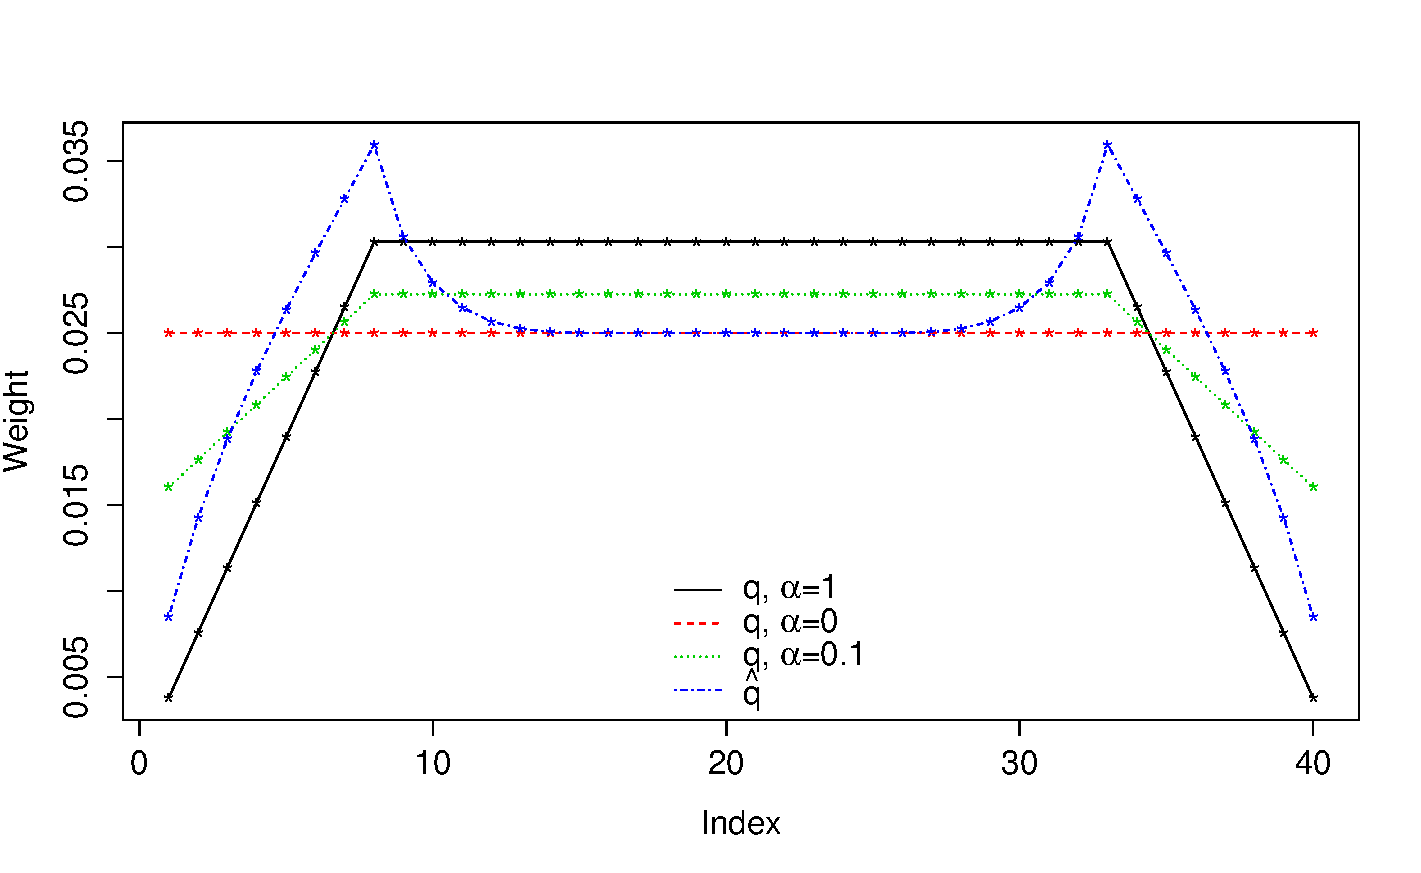
\includegraphics[width = \textwidth]{weights.pdf}\caption{Веса ряда}\label{img_weights}
\end{center}\end{figure}

\subsection{Комментарии к алгоритмам. Сравнение}

Итак, в дальнейшем будем рассматривать и сравнивать методы
Weighted Cadzow, Extended Cadzow, Cadzow ($\alpha$), $0< \alpha \leq 1$, совпадающий с обычным методом Cadzow при $\alpha=1$,
и Cadzow с $\widehat \bfC$.
Заметим, что длина окна $L$ является параметром всех рассматриваемых методов.

\begin{itemize}
\item
Все методы итеративные и, вообще говоря, они не обязаны сходится к глобальному экстремум в задаче МНК  (теоретически, даже сходимость можно иметь место только по подпоследовательностям; однако, во всех проведенных численных экспериментах сходимость имела место). Поэтому сравнение методов, даже
решающих одну и ту же задачу,  по точности имеет смысл.
\item
Сходимость методов по подпоследовательностям имеет место в предположении, что внутренние задачи проектирования в методах Weighted и Extended Cadzow решаются точно. Это напрямую следует из утверждения теоремы \ref{th:converg} для всех методов кроме Extended Cadzow, у которого веса являются частично нулевыми. Однако заметим, что  матрицы $\tilde \bfY_k$, которые содержат столбцы матриц $\Pi_{\calM_r} \bfY_k$ с $L$-го по $N$-ый и каждый элемент которых имеет положительный вес, являются матрицами ранга, не превосходящего $r$, их фробениусова норма не превосходит полунормы исходной матрицы: $\|\tilde \bfY_k\|_F \le \|\Pi_{\calM_r} \bfY_k\|_\bfM$, следовательно, эта ограниченная последовательность и у нее существует сходящаяся к нужному множеству подпоследовательность.
\item
Нас интересует сравнение методов не по достигаемому минимум в задаче МНК, а по точности оценивания выделяемого сигнала $\bfS$.
Вполне возможно, что слишком хорошая аппроксимация исходного ряда может привести к переподгонке, результатом которой
может явиться ухудшение качества оценивания сигнала.
\item
Методы Weighted Cadzow и Extended Cadzow решают задачу \eqref{L-rank_task} c единичными весами $q_i$. Остальные методы решат задачу с весами, отличающимися от равных в той или иной степени.
\item
Однако каждая итерация методов Weighted Cadzow и Extended Cadzow отличается повышенной трудоемкостью, так как использует
еще один итеративный алгоритм на каждой основной итерации.
\item
Трудоемкость методов определяется как трудоемкостью одной итерации, так и числом итераций. Поэтому с этой точки зрения скорость сходимости представляет значительный интерес.
\item
На примере обычного метода Cadzow, известно, что при решении реальных задач одна итерация может представлять значительный интерес, как по трудоемкости, так и по широкому спектру решаемых задач. А именно, одна итерация метода Cadzow --- это известным метод Singular Spectrum Analysis (SSA), который умеет решать существенно большее число задач, чем сам итеративный метод. Поэтому представляет интерес также точность оценивания сигнала, выполненная с помощью одной итерации во всех рассматриваемых методах.
\item
В методе SSA есть понятие разделимости, которое определяет свойство метода (приближенно) находить сигнал по наблюдаемой сумме. Тем самым разделимость
тесно связана с точностью первой итерации итеративного метода. В свою очередь, естественно предположить, что точность первой итерации связана со скоростью сходимости метода. Поэтому вопросы разделимости имеют отношение к скорости сходимости итеративных алгоритмов.
\item
Связь разделимости с длиной окна $L$ для метода SSA хорошо изучена (см., например, \cite{Golyandina2010}). А именно, оптимальная длина окна близка
к половине длины ряда. Маленькие длины окна $L$ приводят к плохой разделимости. Влияние параметра $\alpha$ в классе алгоритмов
Cadzow ($\alpha$) на разделимость исследуется в приложении (раздел~\ref{sec:app}) на примере разделения константы и гармоники. Там показано, что малые значения
$\alpha$ приводят к плохой разделимости, хотя именно они соответствуют примерно равным весам $q_i$ в задаче \eqref{L-rank_task}.
В целом, виден следующий эффект: параметры, соответствующие более равномерным весам, приводят к худшей разделимости.
\item
Вполне возможно, что хорошая скорость сходимости и точность оценивания сигнала являются свойствами, которые не выполняются одновременно, как в силу
противоречия между равномерностью весов и разделимостью, так и потому что медленная сходимость вполне может привести к сходимости алгоритма к лучшему значению оптимизационной задачи.
\end{itemize}

\begin{remark}
\label{rem:adjust}
Во всех алгоритмах к $\widehat\tsS$ можно применить поправку \eqref{eq:adjust}, где $\|\cdot\|$ --- обычная евклидова норма независимо от алгоритма,
так как она согласуется с задачей \eqref{L-rank_task} с равными весами $q_i$.
Полученные алгоритмы будем называть алгоритмами с поправкой.
Например, результат работы $k$-й итерации алгоритма Cadzow можно записать как $\widehat\tsS_k = \calT^{-1}(\Pi_\calH \Pi_{\calM_r})^k \calT \tsX$.
Тогда результат $k$-й итерации алгоритма Cadzow с поправкой имеет вид $\widehat\tsS_k^*=\calA(\widehat\tsS_k)$.
\end{remark}

\section{Численные эксперименты}
\label{sec:simul}
В этом разделе мы приведем численные результаты, призванные продемонстрировать указанные выше выводы и соображения.
Сравнение было проведено для случая выделения синуса и экспоненциально-модулированного синуса.
Так как результаты, в целом, аналогичны, мы приведем только результаты, полученные для выделения гармонического ряда.

Был взят следующий сигнал:
\begin{equation*}
\tsS = (s_{1}, \ldots, s_N), \qquad s_{i} = 5\sin{\frac{2 \pi k}{6}}, \quad k = 1, \ldots, N, \quad N = 40
\end{equation*}
и рассматривался ряд в виде $\tsX = \tsS + \tsN$, где  $\tsN$ --- гауссовский белый шум с математическим ожиданием $0$ и дисперсией, равной $1$.
Точность оценивания сигнала оценивалась с помощью корня из среднего по точкам ряда и по 1000 реализациям ряда среднеквадратического отклонения (CKO)
$\widehat\tsS$ от сигнала $\tsS$.
Эту меру будем называть RMSE (root mean square error) оценки сигнала.
Сравнение проводилось на одних и тех же реализациях исходного ряда. Результаты сравнения являются значимыми
при уровне значимости 5\%.

Рассмотрим сначала класс методов Oblique Cadzow, включающий в себя и обычный метод Cadzow.
Рисунок \ref{img_cadzowspeed2} показывает одновременно скорость сходимости для разных значений параметра $\alpha$ и двух разных длин окна $L$.
По оси x откладывается номер итерации, по оси y --- RMSE оценки сигнала, деленное на число точек в ряде.
\begin{figure}[!hhh]
\begin{center}
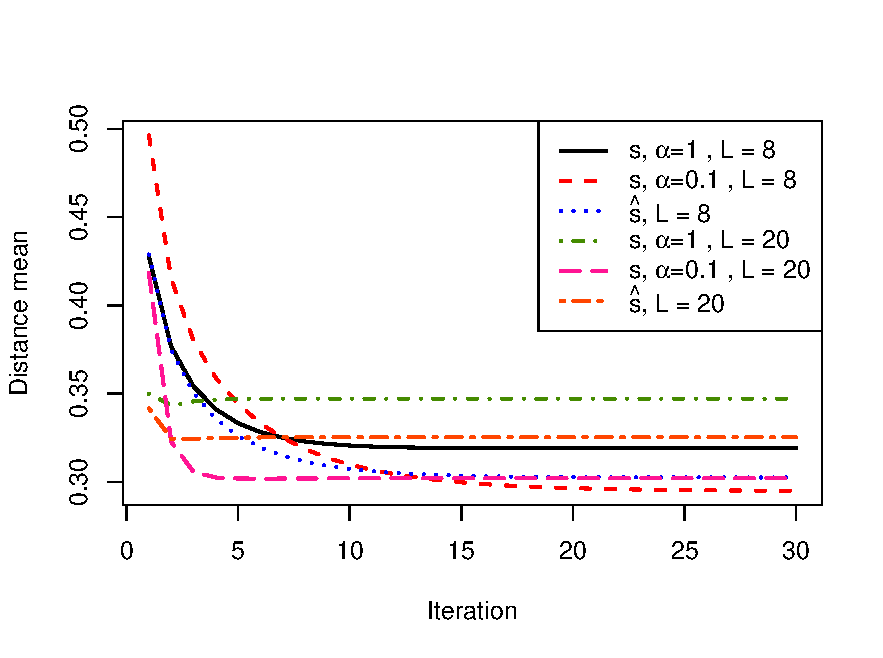
\includegraphics[width = \textwidth]{cadzowspeed_2.pdf}
\caption{RMSE оценки сигнала в зависимости от числа итераций.}
\label{img_cadzowspeed2}
\end{center}
\end{figure}

В пределе самым лучших оказался самый медленно сходящийся метод, а именно, из рассмотренных методов это Cadzow (0.1) с длиной окна $L=8$.
Этот метод также соответствует наиболее равномерным весам из рассматриваемых в примере.
Заметим, что точность всех рассматриваемых методов различается не очень сильно, от 0.33 ($\alpha=0.1$, $L=8$) в лучшем случае до 0.37 в худшем
($\alpha=1$, $L=20$). Однако в первом случае ошибка 0.38 достигается уже на первой итерации, в то время как во втором для
достижения ошибки 0.38 требуется около 4--5 итераций.

Рассмотрим более подробно распределение ошибки по элементам ряда При этом включим в рассмотрение и
методы Extended и Weighted.
В качестве критерия остановки STOP1 для основных итераций будем использовать в алгоритмах число итераций, равное 100 (полученные результаты
можно считать предельными), а для внутренних итераций критерий STOP2 будет иметь вид $\frac{\|\bfY_k - \bfY_{k+1}\|^2}{LK} < 10^{-4}$.
Начальные левые и правые добавленные точки $\tsL_{L-1}$ и $\tsR_{L-1}$
в методе Extended Cadzow строились с помощью векторного SSA прогноза \cite[раздел 2.3.1]{Golyandina.etal2001}.

Возьмем длину окна $L=20$.  На рисунках~\ref{fig:s1_it1}~и~\ref{fig:s1_it100} по оси x откладывается номер точки ряда,
а по оси y --- RMSE от истинного значения сигнала в данной точке. Рисунок~\ref{fig:s1_it1} показывает ошибки на первой итерации,
а рисунок~\ref{fig:s1_it100} --- на итерации с номером 100.
Видно, что в обоих случаях самым точным оказывается метод Extended Cadzow. Из методов, не имеющих внутренних итераций,
на первой итерации выигрывают методы обычный Cadzow и Cadzow c $\widehat\bfC$. В пределе (после 100-й итерации результаты практически не меняются)
наилучшим из них, что не удивительно после анализа рисунка~\ref{img_cadzowspeed2}, оказался Cadzow с $\alpha=0.1$.

\begin{figure}[!hhh]
\begin{center}
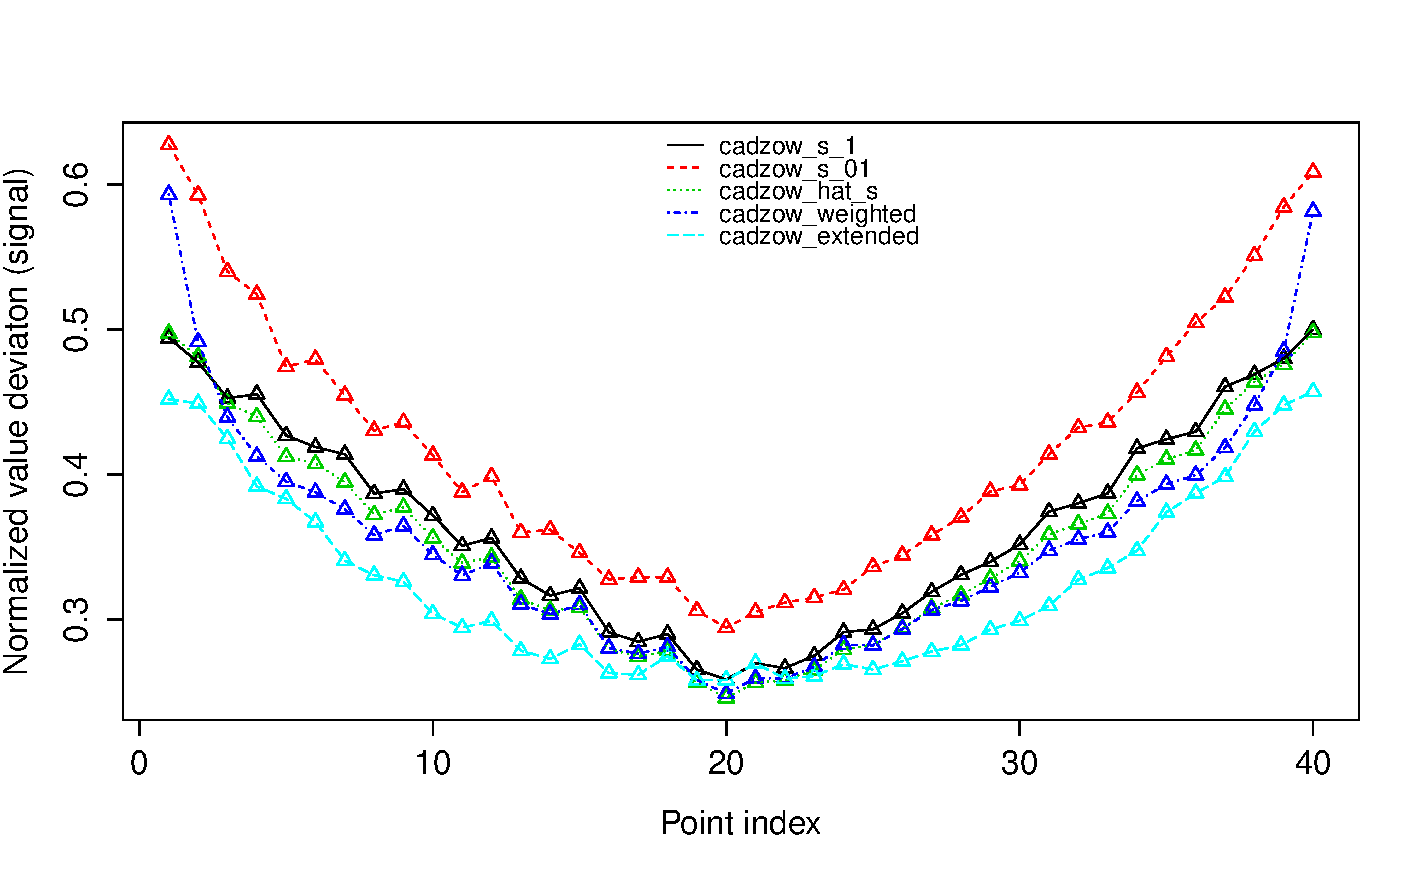
\includegraphics[width = 13cm]{s1_it1.pdf}
\caption{RMSE оценки сигнала в каждой точке ряда на одной итерации.}
\label{fig:s1_it1}
\end{center}
\end{figure}

\begin{figure}[!hhh]
\begin{center}
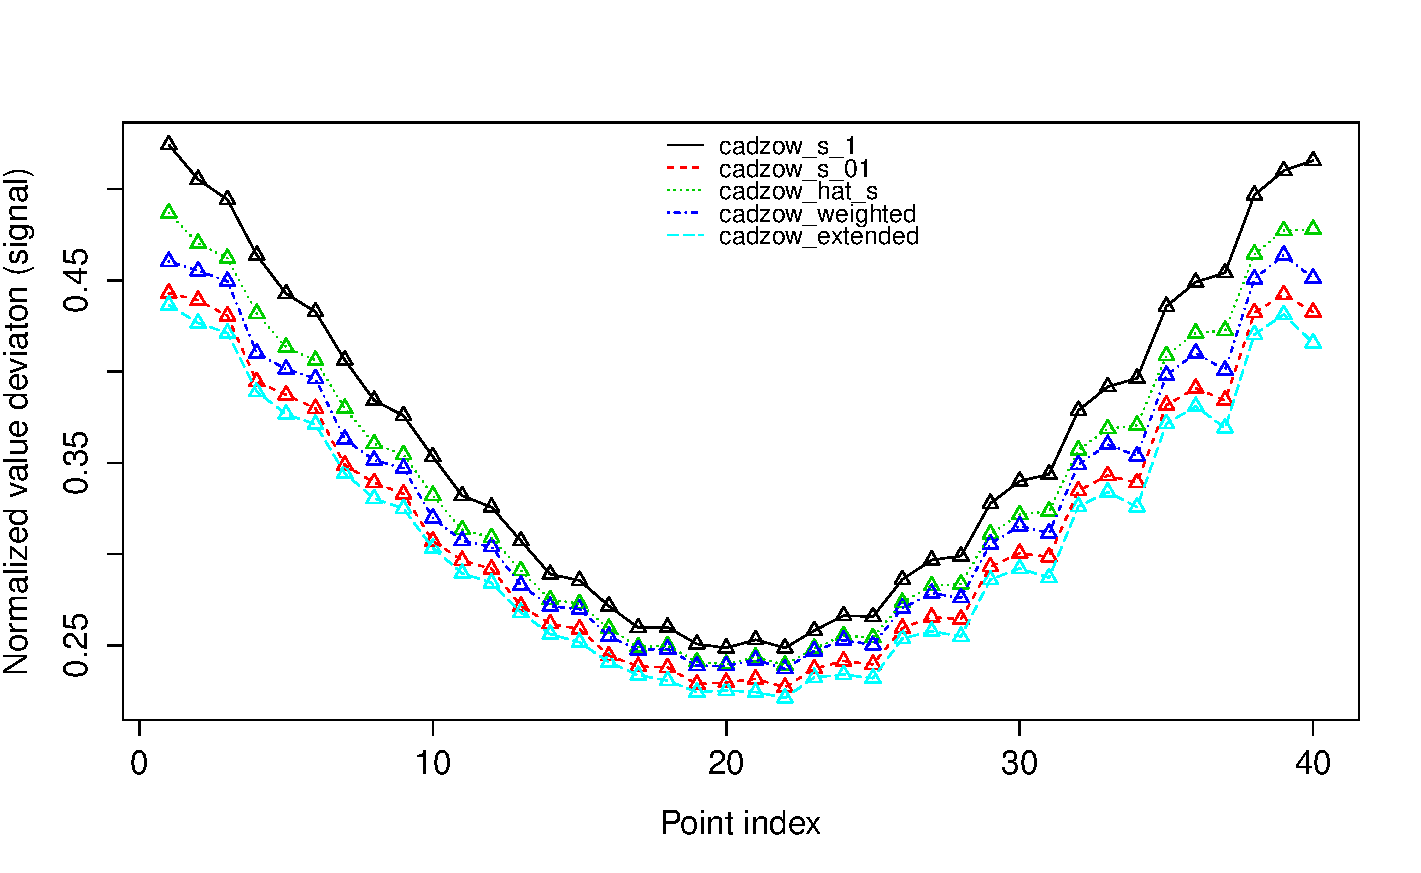
\includegraphics[width = 13cm]{s1_it100.pdf}
\caption{RMSE оценки сигнала в каждой точке ряда на ста итерациях.}
\label{fig:s1_it100}
\end{center}
\end{figure}

Приведем таблицу~\ref{fintable}, где отражены результаты методов, а именно, RMSE как меры отклонения от сигнала и исходного ряда на одной и 100 итерациях.
В таблице $k$ --- число итераций, $\tsS$ --- сигнал, $\tsX$ --- исходный ряд; $L=20$. Таблица подтверждает выводы по сравнению методов по точности
оценивания сигнала. Также видно, что качество аппроксимации исходного ряда не всегда согласуется с качеством оценивания сигнала.
Например, для Cadzow c $\alpha=0.1$ на первой итерации явно видна переподгонка. Однако в пределе упорядоченность точности аппроксимации
и точности оценки сигнала одинаковые.

В таблице \ref{fintable_improved} содержатся аналогичные измерения для рядов с поправкой (см. замечание~\ref{rem:adjust}).
Видно, что поправка влияет незначительно (графики для результатов методов с поправкой мы не приводим, так как визуально влияние поправки незаметно). Аппроксимацию ряда поправка улучшает (не ухудшает) во всех случаях,
как и должно быть по ее построению. На точность оценивания сигнала поправка влияет неоднозначно. На 100-ой итерации она улучшает точность,
а на 1-й результаты разные.

\begin{table}[!hhh]
\begin{center}
\caption{Сравнение алгоритмов по RMSE.}\label{fintable}
\begin{tabular}{|c|c|c|c|c|}
\hline
$P$: & $\tsS$, $k = 1$ & $\tsX$, $k = 1$ & $\tsS$, $k = 100$ & $\tsX$, $k = 100$  \\
\hline
Cadzow, $\alpha = 1$ & 0.3758 & 0.9195 & 0.3782 & 0.9664 \\
\hline
Cadzow, $\alpha = 0.1$ & 0.4329 & 0.7040 & 0.3311 & 0.9506 \\
\hline
Cadzow $\hat{\bfC}$ & 0.3655 & 0.8925 & 0.3559 & 0.9583 \\
\hline
Weighted Cadzow & 0.3644 & 0.8891 & 0.3455 & 0.9549 \\
\hline
Extended Cadzow & 0.3361 & 0.9030 & 0.3189 & 0.9471 \\
\hline
\end{tabular}
\end{center}
\end{table}

\begin{table}[!hhh]
	\begin{center}
		\caption{Сравнение алгоритмов с поправкой по RMSE.}\label{fintable_improved}
		\begin{tabular}{|c|c|c|c|c|}
			\hline
			$P$: & $\tsS$, $T = 1$ & $\tsX$, $T = 1$ & $\tsS$, $T = 100$ & $\tsX$, $T = 100$  \\
			\hline
			Cadzow, $\alpha = 1$ & 0.3714 & 0.9175 & 0.3667 & 0.9622 \\
			\hline
			Cadzow, $\alpha = 0.1$ & 0.4385 & 0.7023 & 0.3276 & 0.9493 \\
			\hline
			Cadzow $\hat{\bfC}$ & 0.3626 & 0.8909 & 0.3478 & 0.9555 \\
			\hline
			Weighted Cadzow & 0.3640 & 0.8883 & 0.3380 & 0.9523 \\
			\hline
			Extended Cadzow & 0.3370 & 0.9030 & 0.3184 & 0.9469 \\
			\hline
		\end{tabular}
	\end{center}
\end{table}

\section{Заключение}
\label{sec:concl}
В работе были рассмотрены известные итеративные алгоритмы и предложены новые для аппроксимации ряда рядами конечного ранга с целью
оценивания сигнала в зашумленном ряде по взвешенному методу наименьших квадратов.


Был рассмотрен довольно широкий набор алгоритмов с целью получить равные веса в МНК. В рассматриваемых алгоритмах равные веса удалось
получить только с помощью вложенных итераций, которые сходятся только к локальному экстремуму и вдобавок делают алгоритм очень трудоемкими.
Итеративные методы без вложенных итераций дают только приближенно равные веса.

Для рассматриваемого класса алгоритмов типа алгоритмов Cadzow была доказана сходимость внешних итераций алгоритмов по подпоследовательностям.

На примере зашумленного синуса с помощью моделирования были получены результаты по точности и скорости сходимости предлагаемых алгоритмов.
Результаты показали, что самым точным оказывается самый трудоемкий метод.
Были рассмотрены вопросы соотношения скорости сходимости, трудоемкости и точности методов.
Акцент был сделан также на точности оценки с помощью одной итерации методов.

В дальнейшем предполагается провести расширенное численное и аналитическое исследование методов и получить более конкретные рекомендации по
соотношению трудоемкости и точности алгоритмов.

%\bibliographystyle{plain}
\bibliographystyle{gost2003}
\bibliography{ssa2012}
\addcontentsline{toc}{section}{Список литературы}

\section{Приложение: Разделимость константы и гармоники для двух алгоритмов Oblique Cadzow}
\label{sec:app}

Введем еще одну характеристику алгоритмов, показывающую, насколько хорошо они раскладывают временной ряд на его аддитивные компоненты. Основным применением описанных алгоритмов является задача оценки сигнала, поэтому данное качество нам важно для получения как можно более точной оценки.

Пусть $\bfC \in \sfR^{K \times K}$ --- симметричная неотрицательно определенная матрица, $\tsX_1$ и $\tsX_2$ ---  два разных временных ряда длины $N$, $\bfX^1$, $\bfX^2$ --- их траекторные матрицы. Тогда \emph{коэффициентом корреляции $i$-го и $j$-го столбца} назовем следующую величину:
\begin{equation}\label{col_corr}
\rho^c_{i,j} = \frac{(X^1_i, X^2_j)}{\|X^1_i\| \|X^2_j\|},
\end{equation}
где $X^k_i$ --- $i$-й столбец матрицы $\bfX^k$, $k = 1, 2$, $(\cdot, \cdot)$ --- евклидово скалярное произведение, $\|\cdot\|$ --- евклидова норма. \emph{Коэффициентом корреляции $i$-й и $j$-й строки} назовем следующую величину:
\begin{equation}\label{row_corr}
\rho^r_{i,j} = \frac{(X^{1,i}, X^{2,j})_\bfC}{\|X^{1,i}\|_\bfC \|X^{2,j}\|_\bfC},
\end{equation}
где $X^{k,i}$ --- $i$-я строчка матрицы $\bfX^k$, $k = 1, 2$, а $(\cdot, \cdot)_\bfC$ --- скалярное произведение с матрицей $\bfC$ в $\sfR^K$, определенная следующим образом: $(X, Y)_\bfC = X \bfC Y^\sfT$, так как $X$, $Y$ --- вектор-строчки, $\| \cdot \|_\bfC$ --- норма, порожденная этим скалярным произведением. Скажем, что ряды $\tsX_1$ и $\tsX_2$ \emph{слабо $\varepsilon$---разделимы}, если
\begin{equation}\label{weak_sep_eq}
\rho = \max\Big(\max_{1 \le i,j \le K}|\rho^c_{i,j}|, \max_{1 \le i,j \le L}|\rho^r_{i,j}|\Big) < \varepsilon.
\end{equation}
Нас будет интересовать порядок $\varepsilon$ при различных матрицах $\bfC$ и рядах $\tsX_1 = (c, c, \ldots)$ --- некоторая константа и $\tsX_2 = (\cos(2 \pi \omega k), k = 1, 2, \ldots)$, а также при различных $L$ и $K$ при условии, что мы будем брать только $N = L + K - 1$ компонент ряда. Когда $\bfC$ единичная матрица, ответ известен: $\varepsilon$ имеет порядок $1/\min(L,K)$, т.е. скорость сходимости имеет порядок $1/N$ при $L$, пропорциональном $N$.
Этот результат может быть найден в \cite[Раздел 6.1]{Golyandina.etal2001}. Он имеет отношение к точности первой итерации метода Cadzow.

В следующем утверждении рассматривается порядок разделимости для алгоритма Cadzow ($\alpha$), введенном в разделе~\ref{sec:cadzow_alpha}.

\begin{proposition}
\label{prop:separ1}
Пусть $\tsX_1 = (c, c, \ldots)$ --- некоторая константа и $\tsX_2 = (\cos(2 \pi \omega k), k = 1, 2, \ldots)$, где $0<\omega <0.5$, $L,K\ra \infty$ так, что $h = h_L = N/L$, где $N=L+K-1$, --- целое, и $\bfC$ определена в алгоритме Cadzow ($\alpha$), т.е.  $\bfC$ --- диагональная матрица со следующими диагональными элементами:
\begin{equation*}
c_k = \begin{cases}
1, & \text{если} \quad k = jL+1 \quad \text{для некоторого} \ j = 0, \ldots, h-1,\\
\alpha, & \text{в противном случае},
\end{cases}
\end{equation*}
где $0 \le \alpha \le 1$. Тогда $\rho$ имеет порядок $\max(\frac{1}{L}, \frac{(1-\alpha)C_{L,K}+\alpha}{(1-\alpha)N/L+\alpha K})$, где порядок $C_{L,K}$
может может меняться от $O(1)$ до $O(N/L)$ в зависимости от того, как $K$ стремятся к бесконечности.
\end{proposition}

\begin{proof5}{\ref{prop:separ1}}
Необходимо оценить порядки следующих величин:
\begin{gather*}
\rho^c_{i,j} = \frac{\sum_{k=j}^{j + L - 1} \cos(2 \pi \omega k)}{\sqrt{L (\sum_{k=j}^{j + L - 1} \cos^2(2 \pi \omega k))}},\\ \rho^r_{i,j} = \frac{\sum_{k=1}^K c_k\cos(2 \pi \omega (j + k - 1))}{\sqrt{(\sum_{k=1}^K c_k) (\sum_{k=1}^K c_k\cos^2(2 \pi \omega (j + k - 1)))}}.
\end{gather*}
Для доказательства используем следующие факты:
\begin{gather*}
\sum_{k=1}^n \cos(ak + b) = \csc(a/2) \sin(an / 2) \cos \left(\frac{an + a + 2b}{2} \right), \\
\sum_{k=1}^n \cos^2(ak + b) = \frac{1}{4}(\csc(a) \sin(2an + a + 2b) -\\ - \csc(a)\sin(a + 2b) + 2n),
\end{gather*}
для любых вещественных $a, b$ и положительного целого $n$.
Таким образом, когда ряд $\tsX_2$ не представляет из себя константу, числитель в $\rho^c_{i,j}$ имеет порядок $O(1)$, а знаменатель --- $O(L)$.
Первая часть доказана, и ее доказательство целиком аналогично случаю, когда $\bfC$ --- единичная матрица.

Для доказательства второй части выделим отдельно сумму по тем $k$, для которых $c_k=1$:
\begin{gather*}
\sum_{k=1}^K c_k\cos(2 \pi \omega (j + k - 1)) = (1-\alpha) \sum_{\substack{1 \le k \le K: \\ c_k = 1}}\cos(2 \pi \omega (j + k - 1)) +\\ +\sum_{1 \le k \le K}\alpha \cos(2 \pi \omega (j + k - 1)) = (1-\alpha) C_{L,K} + \alpha\, O(1),
\\
%\end{gather*}
%\begin{gather*}
\sum_{k=1}^K c_k = (1-\alpha) N/L + \alpha K,
\\
%\end{gather*}
%\begin{gather*}
\sum_{k=1}^K c_k\cos^2(2 \pi \omega (j + k - 1)) = (1-\alpha)\sum_{\substack{1 \le k \le K: \\ c_k = 1}}\cos^2(2 \pi \omega (j + k - 1)) +\\ +\sum_{1 \le k \le K }\alpha \cos^2(2 \pi \omega (j + k - 1)) = (1-\alpha) O(N/L) + \alpha\, O(K).
\end{gather*}
В худшем случае, если $L\omega$ целое, получаем, что $\cos(2 \pi \omega (j + k - 1))$ равно одной и той же константе независимо от $j$ и $k$, и тогда $C_{L,K}$ имеет порядок $O(N/L)$.
\end{proof5}

Таким образом, даже в лучшем случае, когда $C_{L,K}$ имеет порядок $O(1)$, разделимость константы и синуса становится хуже, чем при обычном варианте: при $\alpha$, близких к нулю, оптимальным выбором $L$ будет $L \approx \sqrt{N}$, и, таким образом, получаем порядок разделимости $1/\sqrt{N}$.

Теперь рассмотрим алгоритм Cadzow с $\widehat\bfC$, введенный в разделе~\ref{sec:cadzow_hat}.

\begin{proposition}
\label{prop:separ2}
Пусть $\tsX_1 = (c, c, \ldots)$ --- некоторая константа и $\tsX_2 = (\cos(2 \pi \omega k), k = 1, 2, \ldots)$, где $0<\omega <0.5$, $L,K\ra \infty$ и $\bfC$ определена в алгоритме Cadzow с $\widehat\bfC$.
 Тогда $\rho$ имеет порядок $\max \left(1/L, \frac{H_L}{\sqrt{NK}} \right)$ при $L, K \to \infty$, где $H_L$ --- $L$-е гармоническое число.
\end{proposition}

\begin{proof5}{\ref{prop:separ2}}
Необходимо оценить порядки следующих величин:
\begin{gather*}
\rho^c_{i,j} = \frac{\sum_{k=j}^{j + L - 1} \cos(2 \pi \omega k)}{\sqrt{L (\sum_{k=j}^{j + L - 1} \cos^2(2 \pi \omega k))}}, \\ \rho^r_{i,j} = \frac{\sum_{k=1}^K \hat c_k\cos(2 \pi \omega (j + k - 1))}{\sqrt{(\sum_{k=1}^K \hat c_k) (\sum_{k=1}^K \hat c_k\cos^2(2 \pi \omega (j + k - 1)))}}.
\end{gather*}
 Порядок $\rho^c_{i,j}$ уже был получен в доказательстве предложения~\ref{prop:separ1}, поэтому сразу перейдем к $\rho^r_{i,j}$. Рассмотрим корреляцию только первых строчек --- для остальных доказательство будет целиком аналогичным. Рассмотрим числитель $\rho^r_{1,1}$:
\begin{gather*}
\sum_{k=1}^K \hat c_k\cos(2 \pi \omega k) = \sum_{k=1}^{L-1} \hat c_k\cos(2 \pi \omega k) + \sum_{k=L}^{K - L + 1} \frac{\cos(2 \pi \omega k)}{L} +\\+ \sum_{k=K - L + 2}^{K} \hat c_k\cos(2 \pi \omega k) = I_1 + I_2 + I_3,
\end{gather*}
который разбился на три части. Для $I_2$ справедлива оценка $O(1/L)$, а для $I_3$ доказательство аналогично доказательству для $I_1$:
\begin{gather*}
|I_1|=\bigg|\sum_{k=1}^{L-1}\frac{1}{L}\left(\frac{k}{L} + \sum_{j=k}^{L-1} \frac{1}{j} \right) \cos(2 \pi \omega k)\bigg| =\\= \bigg|\sum_{k=1}^{L-1} \frac{k \cos(2 \pi \omega k)}{L^2} +  \frac{1}{L}\sum_{k = 1}^{L-1}\sum_{j = k}^{L-1}\frac{\cos(2 \pi \omega k)}{j}\bigg| \le \\ \le
\bigg|\sum_{k=1}^{L-1} \frac{k \cos(2 \pi \omega k)}{L^2}\bigg| + \bigg|\frac{1}{L}\sum_{k = 1}^{L-1}\sum_{j = k}^{L-1}\frac{\cos(2 \pi \omega k)}{j}\bigg|.
\end{gather*}
Используя тот факт, что
\begin{gather*}
\sum_{k=1}^n k \cos(ak + b) = -\frac{1}{4}\csc^2(a/2)(-(n+1)\cos(an+b) + \\ + n\cos(an + a + b) + \cos b),
\end{gather*}
получаем:
\begin{gather*}
\bigg|\sum_{k=1}^{L-1} \frac{k \cos(2 \pi \omega k)}{L^2}\bigg| = O(1/L), \quad
\bigg|\frac{1}{L}\sum_{k = 1}^{L-1}\sum_{j = k}^{L-1}\frac{\cos(2 \pi \omega k)}{j}\bigg| = \\ =\bigg|\frac{1}{L}\sum_{j = 1}^{L-1}\sum_{k = 1}^{j}\frac{\cos(2 \pi \omega k)}{j}\bigg| \le \bigg|\frac{1}{L}\sum_{j = 1}^{L-1}\frac{d}{j}\bigg| = O \left(\frac{H_L}{L} \right),
\end{gather*}
где $d$ --- некоторая константа. 

Для знаменателя нужно рассмотреть следующие суммы:
\begin{equation*}
\sum_{k=1}^K \hat c_k = N / L
\end{equation*}
по определению, а следующую составляющую просто оценить снизу:
\begin{equation*}
\sum_{k=1}^K \hat c_k\cos^2(2 \pi \omega (j + k - 1)) \ge \sum_{k=1}^K \frac{1}{L}\cos^2(2 \pi \omega (j + k - 1)) = O \left(\frac{K}{L} \right).
\end{equation*}
\end{proof5}


\end{document}
